%\begin{filecontents*}{MIRSVM.eps}
%gsave
%newpath
%  20 20 moveto
%  20 220 lineto
%  220 220 lineto
%  220 20 lineto
%closepath
%2 setlinewidth
%gsave
%  .4 setgray fill
%grestore
%stroke
%grestore
%\end{filecontents*}
\RequirePackage{fix-cm}
\documentclass[smallcondensed]{svjour3}                 
\smartqed  
\hyphenation{op-tical net-works semi-conduc-tor}
\usepackage[hidelinks]{hyperref}
\usepackage{amsmath,amssymb,mathtools,float,times,bm,tikz,proof,tabularx,capt-of,natbib}
\usepackage{graphicx,amsfonts,array,url,algorithm,algorithmicx,algpseudocode,booktabs}
\usepackage[flushleft]{threeparttable}
\usepackage[top=1in,bottom=1in,right=1in,left=1in]{geometry}
\usepackage{tikz-cd,adjustbox}
\usetikzlibrary{shapes.geometric,arrows,automata,positioning}
\usepackage{setspace}
\let\Algorithm\algorithm
\renewcommand\algorithm[1][]{\Algorithm[#1]\setstretch{1}}

\newcommand{\iitem}{\item[-]}
\newcommand{\set}[1]{{\left\{#1\right\}}} 
\newcommand{\norm}[1]{{||#1||}} 
\newcommand{\st}{{\,|\,}} 
\newcommand{\reals}{{\mathbb R}}
\newcommand{\ints}{{\mathbb Z}}
\newcommand{\spa}[1]{\mathcal{#1}}
\newcommand\tab[1][1cm]{\hspace*{#1}}

\overfullrule=5pt

\journalname{Machine Learning}

\begin{document}

\tikzstyle{decision} = [diamond, draw, text centered, inner sep=3pt]
\tikzstyle{block} = [rectangle, draw, fill=gray!20,text width=5em, text centered, rounded corners, minimum height=4em]
\tikzstyle{arrow} = [thick,->,>=stealth]

\title{MIRSVM: Multi-Instance Support Vector Machine with Bag Representatives}

\author{Gabriella Melki \and
        Alberto Cano			\and
        Sebasti\'an Ventura
}

\institute{Gabriella Melki \at
			Virginia Commonwealth University, 401 W. Main St. E2264, Richmond, VA 23284\\
            \email{melkiga@vcu.edu}          
           \and
           Alberto Cano \at
           	Virginia Commonwealth University, 401 W. Main St. E4251, Richmond, VA 23284\\
            \email{acano@vcu.edu}
           \and
           Sebasti\'an Ventura \at
            University of C\'{o}rdoba, ``Albert Einstein Building'', 3rd floor, 14071 C\'{o}rdoba, Spain\\
            \email{sventura@uco.es}
}

\date{Received: date / Accepted: date}
% The correct dates will be entered by the editor

\maketitle

\begin{abstract}
\textit{Multiple-instance learning} (MIL) is a generalization of \textit{supervised learning}, where samples are represented by labeled bags, each containing sets of instances. The individual labels of the samples within a bag are unknown, and labels are assigned based on a multi-instance assumption. One of the major complexities associated with this type of learning is the ambiguous relationship between a bag's label and the instances it contains. This paper proposes a novel support vector machine (SVM) multiple-instance formulation and presents an algorithm with a bag-representative selector that trains the SVM based on bag-level information, named MIRSVM. The contribution is able to identify instances that highly impact classification, i.e. bag-representatives, for both positive and negative bags, while finding the optimal class separation hyperplane. Unlike other multi-instance SVM methods, this approach eliminates possible class imbalance issues by allowing both positive and negative bags to have at most one representative, while highlighting the instances that contribute most to the classification model. The experimental study evaluates and compares the performance of this proposal against $10$ state-of-the-art multi-instance methods over $15$ datasets, and the results are validated through non-parametric statistical analysis. The results indicate that bag-based learners outperform the instance-based and wrapper methods, as well as this proposal's overall superior performance against other multi-instance SVM models. 
\keywords{Machine learning \and multiple-instance learning \and support vector machines \and bag-level multi-instance classification \and bag-representative selection}
\end{abstract}

\section{Introduction}\label{intro}
In traditional classification, learning algorithms attempt to correctly label unknown samples by finding patterns that exist between training samples and their class label. \textit{Multi-instance} (MI) learning (or \textit{multiple-instance} learning) is a generalization of \textit{supervised learning} that has been recently been gaining interest because of its applicability to many real-world problems such as text categorization \citep{Andrews2002}, image classification \citep{Herman2008,Wei2016155}, human action recognition \citep{Yi2016}, and drug activity prediction \citep{Dietterich1997}. 

The difference between MIL and traditional learning is the nature of the data samples. In the traditional setting, each sample is represented by a single feature vector that has its own class label. In multi-instance learning, a sample is considered to be a \textit{bag} that contains multiple instances, and is associated with a single label. The individual labels of the samples within a bag, referred to as \textit{instances}, are unknown, and labels are assigned based on a multi-instance assumption, or hypothesis. Introduced by~\cite{Dietterich1997}, the standard MI assumption states that a bag is labeled as positive if and only if it contains at least one positive instance. More recently, other MI hypotheses and frameworks have been proposed by~\cite{Foulds2010} to encompass a wider range of applications with multi-instance data. 

One of the major complexities associated with multi-instance learning is the ambiguity of the relationship between a bag label and instances within the bag~\citep{Alpaydin2015}. This stems from the standard MIL assumption, where the underlying distribution among instances within positive bags is unknown. All that is known is that at least one instance has a positive label within a positive bag. There have been different attempts to overcome this complexity. One approach involves ``flattenning" the MIL datasets, meaning samples contained in positive bags each adopt a positive label, allowing the use of classical supervised learning techniques~\citep{Ray2005}. This approach assumes that positive bags contain a significant number of positive samples, which may not be the case, causing the classifier to mislabel negative instances within the bag, decreasing the power of the resulting MIL model. 

To overcome this, a different MIL approach was proposed, where subsets of instances are selected from positive bags for classifier training~\citep{Maron1998,Zhang2001}. One drawback of this type of method is that the resulting training datasets become imbalanced towards positive instances by significantly decreasing the number of negative instances. The performance of these methods deteriorates when more instances are selected as subsets than needed~\citep{Carbonneau2016,Faria2017196,Vanwinckelen2016}. Our proposal aims to deal with this drawback by minimizing class imbalance. This is achieved by optimally selecting bag-representatives from both classes using Support Vector Machines.

Support Vector Machines (SVMs) represent a set of supervised, linear and nonlinear, classification and regression methods that have theoretical foundations on Vapnik-Chervonenkis (VC) theory~\citep{Huang2006,Schoelkopf2002}. SVM models are similar to other machine learning algorithms and techniques, but research has shown that they usually outperform them in terms of computational efficiency, scalability, and robustness against outliers~\citep{Kecman2016,Melki2016}, which makes them a useful data mining tool for various real-world applications. 

To address the limitations presented by MIL algorithms, this paper proposes a novel support vector machine formulation with a bag-representative selector, called Multiple-Instance Representative Support Vector Machine (MIRSVM). SVMs are known to perform well when data is limited, therefore combining them with a bag-representative selector aims to remedy class imbalance caused by limited positive bags, without assuming their internal distributions. The algorithm selects bag-representatives iteratively according to the standard MI assumption, ensuring known information, such as the negative bag labels, are fully utilized during the training process. The optimal separating hyperplane between bags is then found with respect to the bag-representatives using a Gaussian kernel and a quadratic programming solver. The optimal set of representatives is found when they have stopped changing from one iteration to the next. The algorithm does not assume any distribution of the instances and is not affected by the number of samples within a bag, making it applicable to a variety of contexts. The key contributions of this work include,
\begin{itemize}
\iitem Reformulating the traditional primal L$1$-SVM problem to optimize over bags, rather than instances, ensuring all the information contained within each bag is utilized during training, while defining bag representative selector criteria.

\iitem Deriving the dual multi-instance SVM problem, with the Karush-Kuhn-Tucker necessary and sufficient conditions for optimality. The dual is maximized with respect to the Lagrange multipliers and provides insightful information about the resulting sparse model. The dual formulation is kernelized with a Gaussian radial basis function, which calculates the distances between bag representatives.

\iitem Devising a unique bag-representative selector method that makes no presumptions about the underlying distributions of the instances within each bag, while maintaining the default MIL assumption. This approach eliminates the issue of class imbalance caused by techniques such as flattening or subsetting positive instances from each bag. The key feature of MIRSVM is its ability to identify instances (support vectors) within positive and negative bags that highly impact the model.
\end{itemize}

This work is organized as follows. First, the notation used throughout the paper is provided, the MIL problem is formalized, and recent multiple-instance learning methods, traditional support vector machines, and state-of-the-art multi-instance SVM methods are reviewed in Section~\ref{sec:background}. The primal L$1$-SVM is formulated with respect to optimizing over bags, the dual formulation is then derived, along with the conditions for optimality, and the proposed algorithm, MIRSVM, is listed and described in Section~\ref{sec:contribution}. Section~\ref{sec:experiments} presents the experimental environment, including results from various metrics, run-time, and non-parametric statistical analysis over $15$ benchmark MI datasets compared with $10$ state-of-the-art algorithms. Finally, Section~\ref{sec:conclusion} presents the conclusions of this contribution.

\section{Background}\label{sec:background}
This section defines the notation that will be used throughout the paper, and reviews related works on multi-instance learning, traditional support vector machines, and multi-instance support vector machines.

\subsection{Notation}\label{subsec:notation}
Let $\mathcal{D}$ be a training dataset of $n$ bags. Let $\bm{Y} \in \mathcal{D}$ be a vector of $n$ labels corresponding to each bag, having a domain of $\bm{Y} \in \set{-1,\,+1}^n$. Let $\bm{X} \in \mathcal{D}$ be a matrix consisting of $d$ input variables and $m$ instances, having a domain of $\bm{X} \in \mathbb{R}^{m \times d}$. Let $\bm B$ be the set of bags which contain a number of instances, sometimes of different size, and usually non-overlapping, such as $\bm{B}_I = \{\bm x_{1}, \ldots, \bm x_{|\bm B_I|}\}$ for index set $I \subseteq \set{1,\ldots,n}$, where $|\bm B_I|$ is the number of instances in bag $I$. Using the training dataset $\mathcal{D} = \{(\bm B_1,Y_1), \ldots, (\bm B_n,Y_n)\}$, the goal is to learn a model $f : \bm{X} \times Y$, that assigns a label, $Y_I \in \set{-1,\,+1}$, for each input bag $\bm{B}_I$. The model will then be used to predict the labels of new, unlabeled, and unseen input bags. Table~\ref{tab:Notation} provides a summary of the notation used in this paper.
\begin{table}
\caption{Summary of notation used throughout the paper}\label{tab:Notation}
\begin{tabularx}{\textwidth}{l@{\extracolsep{\fill}}l}
\hline\noalign{\smallskip}
Definition & Notation\\ 
\noalign{\smallskip}\hline\noalign{\smallskip}
Number of Bags & $n$ \\
Number of Instances & $m$ \\
Number of Input Attributes & $d$ \\
Set of Bags & $\bm B = \set{\bm B_1,\, \ldots,\, \bm B_n}$ \\
Bag Index Set & $I \in \ints_+^n$ \\
Input Space & $\bm{X} \in \mathbb{R}^{m \times d}$ \\
Bag $I$ & $\bm B_I = \set{\bm x_i \st \forall i \in I}$ \\
Input Instance $i$ from Bag $I$ & $\bm{x}_i = (x_{1}, \ldots, x_{d}),\, i \in I$ \\
Bag Labels & $\bm{Y} \in \{-1,\,1\}^n$ \\
Individual Instance Label $i$ & $y_i \in \set{-1,+1}$ \\
\noalign{\smallskip}\hline\noalign{\smallskip}
Full Multi-Instance Training Dataset & $\mathcal{D} = \{(\bm B_1,Y_1), \ldots, (\bm B_n,Y_n)\}$ \\
Full Single-Instance Training Dataset & $\mathcal{S} = \{(\bm x_1,y_1), \ldots, (\bm x_m,y_m)\} $\\
\noalign{\smallskip}\hline
\end{tabularx}
\end{table}

\subsection{Multiple-Instance Learning}\label{subsec:mil}
In traditional binary classification problems, the goal is to learn a model that maps input samples to labels, $f: \reals^{m \times d} \rightarrow Y^m \in \set{-1,\,+1}$. Multiple instance learning generalizes this framework and makes weaker assumptions about sample labeling. In the MIL case, samples are called \textit{bags} and each bag contains one or more input instances. Each bag is assigned a label, unlike traditional classification problems, where individual samples are assigned a label. Input instances, $\set{\bm x_1,\, \bm x_2,\, \ldots,\, \bm x_m}$, are grouped into bags with unique identifiers, $\bm B = \set{\bm B_1,\, \bm B_2,\, \ldots,\, \bm B_n \st \bm B_I = \set{\bm x_i \st \forall i \in I}}$, $\forall I \in \set{1, \ldots, n}$ and assigned a label, $Y_I$. An example representation of an MI dataset is shown in Figure~\ref{fig:mirep}. 

In MIL, the goal is to train a classifier that predicts the label of an unseen bag, $f(\bm B_{n+1}) \rightarrow Y_{n+1}$~\citep{Amores2013}. In order to build a classifier without any knowledge of the individual training instance labels,~\cite{Dietterich1997} proposed the \textit{standard MI} (SMI) hypothesis based on the domain of drug-activity prediction, shown in Equation~\ref{eqn:stas}, which states that a bag is labeled positive if and only if at least one of the instances in the bag is positive, and is labeled negative otherwise.
\begin{equation}
\centering \label{eqn:stas}
 Y_I = \begin{cases}
			+1 & \text{if }\exists\, y_i = +1,\, \forall i \in I \\
			-1 & \text{otherwise}.
		  \end{cases}
\end{equation}

This implies that individual instance labels $y_i$ exist, but are not known during training. Equation~\ref{eqn:stas} can also be rewritten as Equation~\ref{eqn:stasmax} for simplicity:
\begin{equation}
\centering \label{eqn:stasmax}
Y_I = \text{argmax}_{\forall i \in I}\,\,\, y_i.
\end{equation}

In addition to the SMI assumption, alternative MI assumptions have been proposed to date~\citep{Foulds2010}. A recent review describing the taxonomy of multi-instance classification was presented by~\cite{Amores2013}. The review presents various methods and algorithms used in literature which are categorized based on their approach to handling the MI input space. Instance-based classifiers that fall under the \textit{instance-space paradigm}, aim to separate instances in positive bags from those in negative ones. Bag-level classifiers (\textit{bag-space paradigm}) treat each bag as a whole entity, implicitly extracting information from each bag in order to accurately predict their labels. Methods that fall under the \textit{embedded-space paradigm} map the input bags to a single feature vector that explicitly encapsulates all the relevant information contained within each bag.

Instance-based methods that follow the SMI assumption attempt to identify desirable instance properties that make a bag positive. One traditional method in this category is the Axis-Parallel Rectangle (APR)~\citep{Dietterich1997}, which trains a model that assigns a positive label to an instance if it belongs to an axis-parallel rectangle in feature space, and assigns a negative label otherwise. The APR is optimized by maximizing the number of positive bags in the training set containing at least one instance in the APR, while concurrently maximizing the number of negative bags that do not contain any instance in the APR. Another similar method is the Diverse Density (DD)~\citep{Maron1998} framework which is maximized for instances in feature space that are near at least one instance in a positive bag and far from all instances in negative bags. In the Expectation-Maximization Diverse Density (EM-DD) algorithm,~\cite{Zhang2001} propose a similar framework that iteratively maximizes the DD measure.~\cite{Auer2004} present a boosting approach~\citep{Schapire19981651} that uses balls centered around positive bags to solve the MI problem called Multi-Instance Optimal Ball (MIOptimalBall). This approach is similar to that of APR and DD, except that~\cite{Auer2004} propose computing optimal balls per positive bags. A major challenge affecting these methods is that the distributions of the positive and negative bags affect their performance. Methods based on the DD metric~\citep{Chen2004,Chen2006,Carbonneau2016,Zhang2001} assume the positive instances form a cluster, which may not be the case. Alternatively~\cite{Fu2011} models the distribution of negative bags with Gaussian kernels, which can prove difficult when the quantity of data is limited. 
\begin{figure*}
\centering
\begin{tabular}{|c|ccccc|c|}
\hline
$\bm B$ & $F_1$ & $F_2$ & $F_3$ & \ldots & $F_d$ & $Y$ \\        
\hline
    	  & 0.1 & 0.8 & 2.5 & \ldots & 0.8 &    \\        
    $B_1$ 	  & 0.2 & 2.0 & 5.5 & \ldots & 3.0 & POS \\
    	  & 0.1 & ?   & 4.5 & \ldots & 0.1 &    \\
\hline
    	  & 1.5 & 4.0 & 0.8 & \ldots & 0.1 &    \\
    	  & 0.8 & 0.4 & 2.9 & \ldots & 1.1 &    \\
    $B_2$	  & 2.3 & 0.2 & 4.0 & \ldots & 5.5 & NEG \\
    	  & 6.7 & 5.0 & ?   & \ldots & 0.5 &    \\
    	  & 0.1 & 4.0 & 8.7 & \ldots & 3.3 &    \\
\hline
  \end{tabular}
  \caption{Example of multi-instance data representation. The figure shows a sample binary MI dataset with $2$ bags, identified as $B_1$ and $B_2$. The bags each contain differing number of instances, each with $d$ dimension, and are assigned positive and negative labels indicated by column $Y$. Missing instance feature values are denoted by a question mark.}%
  \label{fig:mirep}%
\end{figure*}

Some methods in literature~\citep{Ray2005,Viola2005}, such as Simple-MI~\citep{Dong2006}, transform the MI dataset to a traditional instance-level dataset. Simple-MI represents each bag with the mean vector of the instances within it. This approach was evaluated by~\cite{Bunescu2007} and they proposed mapping each bag to a max-min vector, a concatenation of the features with the highest and lowest values. The major disadvantage of these types of approaches is that they assume the distribution the instances in positive bags is positive, when it may not be.

An extension of traditional single-instance $k$-nearest neighbors method (KNN) was proposed by~\cite{Wang2000} to be applied to the bag-level, named CitationKNN. This method uses a distance function between bags in order to determine bag similarities. Not only are the set of closest bags to a single bag  considered, but also how many bags is the single bag closest to. A voting scheme is then used to determine the bag class labels.~\cite{Xu2011} proposed a multi-instance Decision-Based Neural Network (MI-DBNN), a probabilistic variant of the traditional DBNN, which is a neural network with a modular structure~\citep{Herrera2016}.

~\cite{Blockeel2005} introduced the Multi-Instance Tree Inducer (MITI), based on the standard MI assumption, which uses decision trees as a heuristic to solve the MI problem. This approach aims to identify whether an instance within a bag is truly positive and eliminate false positives within the same bag. The disadvantage of this approach stems from removing instances considered as false positives from partially grown trees without updating the existing tree structure.~\cite{Bjerring2011} then enhanced this approach by creating the method Multi-Instance Rule Induction (MIRI). The algorithm aims to eliminate any possibility of a suboptimal split because the tree is discarded and regrown. Other popular methods include MIBoost~\citep{Hall2009}, MIWrapper~\citep{Hall2009}, and Two-Level Classifier (TLC)~\citep{Wang2014}.

For most of the methods described above, implicit or explicit assumptions have been made about the distribution of the data. Selecting a method that is robust for a problem such as MIL can be difficult when little is known about the nature of the data, especially considering the unknown distribution of the instances within bags~\citep{2015-KAIS,2016-INS-MIARM}. The proposed method, MIRSVM, is a general method that uses support vector machines to design a MIL model without making prior assumptions about the data. Classifiers of this type are known to provide better generalization capabilities and performance, as well as sparser models.

\subsection{Support Vector Machines}\label{subsec:svms}
Most classical machine learning techniques require knowledge of the data distribution in order to learn accurate models~\citep{Alabdulmohsin2016215,Suzumura20171}. This is a serious restriction because, in most cases, the distribution of the data is unknown. Another disadvantage of these methods stems from high dimensional, sparse datasets, which are very common in real-world applications~\citep{durrant2015random}. Small sample size also poses problems of model reliability, especially when coupled with high dimensional feature spaces. SVMs represent learning techniques that have been introduced under the \textit{structural risk minimization} (SRM) framework and VC theory~\citep{Kecman2001}. Rather than optimizing over L1 or L2 norms and classification error, SVMs perform SRM~\citep{Shalev2014}, minimizing the expected probability of classification error, resulting in a generalized model without making assumptions about the data distribution~\citep{Cortes1995}. 

SVMs are a particularly useful for learning linear predictors in high dimensional feature spaces, which is a computationally complex learning problem. In the context of classification, this problem is approached by searching for the optimal \textit{maximal margin} of separability between classes. A training set $\mathcal{D}$ is \textit{linearly separable} if a halfspace exists, $(\bm{w},b)$, such that $y_i = \text{sign }(\langle \bm{w},\bm{x}_i\rangle+b), \forall i \in \{1,\ldots,m\}$, where $\bm w \in \reals^d$ is a $d$-dimensional weight vector, and $b \in \reals$ is a bias term. All halfspaces, defined as $d(\bm{x}_i) = \langle \bm{w},\bm{x}_i\rangle + b$, satisfying $y_i \left(\langle \bm{w},\bm{x}_i\rangle + b\right) > 0,\,\, \forall i \in \{1,\ldots,m\}$, have no error. This hard constraint is associated with the \textit{Hard-Margin SVM}. No feasible solution exists for the Hard-Margin SVM problem if the dataset is non-linearly separable, which is the case for most datasets. To overcome this,~\cite{Cortes1995} introduced the \textit{Soft-Margin L$1$-SVM}:
\begin{subequations} 
\label{eq:primalsvm}
\begin{alignat}{2}
\min\limits_{\bm w,b,\bm\xi}& {\,\,} \frac{1}{2}||\bm{w}||^2 + \frac{C}{m}\sum_{i=1}^m \xi_i \tag{\ref{eq:primalsvm}} \\ 
\text{s.t.}& {\,\,} y_i(\langle\bm{w},\bm{x}_i\rangle + b) \geq 1 - \xi_i,\,\, \forall i \in \{1,\ldots,m\}  \\
{} & {\,\,} \xi_i \geq 0,\,\, \forall i \in \{1,\ldots,m\},
\end{alignat}
\end{subequations} 
where $C \in \reals$ is the penalty parameter that controls the trade-off between margin maximization and classification error minimization, penalizing large norms and errors. The slack variable $\bm \xi \in \reals^m$ allows for optimizing over sample errors. The resulting hyperplane is called \textit{soft-margin hyperplane}. Although the Soft-SVM learns an optimal hyperplane, if the training data set is not linearly separable, the classifier learned may not have a good generalization capability~\citep{Nocedal2006}. Generalization and linear separability can be enhanced by mapping the original input space to a higher dimensional dot-product space by using a kernel function shown in Equation~\ref{eqn:kerneltrick}:
\begin{equation}
\spa{K}\left(\bm{x}_i,\bm{x}_j\right) = \langle \phi\left(\bm{x}_i\right),\,\phi\left(\bm{x}_j\right)\rangle,
\label{eqn:kerneltrick}
\end{equation}
where $\phi\left(\cdot\right)$ represents a function mapping from the original feature space to a higher dimensional space. This kernel mapping is particularly helpful when solving the dual SVM optimization problem shown in Equation~\eqref{eq:dualsvm}. Rather than calculating the inner product of two mapped vectors, their corresponding \textit{scalar} kernel value can be used. 
\begin{subequations}
\label{eq:dualsvm}
\begin{alignat}{2}
\max\limits_{\bm \alpha} &\,\,\,\, \frac{1}{2}\sum_{i,j=1}^m{\alpha_i \alpha_jy_iy_j\spa{K}\left(\bm{x}_i,\bm{x}_j\right)} - \sum_{i=1}^m \alpha_i \tag{\ref{eq:dualsvm}} \\ 
\text{s.t.} &\,\,\,\, \sum_{i=1}^m \alpha_iy_i = 0,  \\
&\,\,\,\, 0 \leq \alpha_i \leq \frac{C}{m},\,\, \forall i \in \{1,\ldots,m\}. 
\end{alignat}
\end{subequations}

A traditional and widely used method of solving the L1-SVM problem is the \textit{Sequential Minimal Optimization} (SMO) technique proposed by~\cite{Platt1998}. It is an iterative procedure that divides the SVM dual problem into a series of sub-problems, which are then solved analytically by finding the optimal $\bm \alpha$ values that satisfy the Karush-Kuhn-Tucker (KKT) conditions~\citep{Boyd2004}. Although SMO is guaranteed to converge, heuristics are used to choose $\bm \alpha$ values in order to accelerate the convergence rate. This is a critical step because the convergence speed of the SMO algorithm is highly dependent on the dataset size, as well as the SVM hyperparameters~\citep{Schoelkopf2002}. \textit{Iterative Single Data Algorithm} (ISDA)~\citep{Huang2006,Kecman2016} is a more recent and efficient approach for solving the L2-SVM problem, shown to be faster than the SMO algorithm and equal in terms of accuracy~\citep{Kecman2015,Kecman2014}. It iteratively updates the objective function by working on one data point at a time, using coordinate descent to find the optimal objective function value. Other methods for solving the SVM problem include \textit{Quadratic Programming} solvers, such as the interior point method. These types of algorithms find the true optimal objective function value at the trade-off of having a relatively slower run-time.

\subsection{Multiple-Instance Support Vector Machines}
The MI adaptation of the SVM presents two contexts for solving the problem: the instance-level and the bag-level. The first tries to identify instances, either all within a bag or just key instances, that help find the optimal separating hyperplane between positive and negative bags. The latter uses kernels defined over whole bags to optimize the margin~\citep{Doran201479}. 

\cite{Andrews2002} proposed a mixed-integer quadratic program that solves the MI problem at an instance-level, using a support vector machine, named MISVM, that can be solved heuristically. Rather than maximizing the margin of separability between instances of different classes, this instance-based method maximizes the margin between bags. It tries to identify the key instance from each positive bag that makes the bag positive by assuming it has the highest margin value~\citep{Herrera2016}. Instances from positive bags are selected as bag-representatives, and the algorithm iteratively creates a classifier that separates those representatives from all instances from the negative bags. Using bag-representatives from one class and all instances from the other is an example of an approach that combines rules from the SMI assumption and the collective assumption. A disadvantage of this approach stems from the assumption that all instances within positive bags are also positive, which is an implicit step in the initialization of MISVM.~\cite{Andrews2002} also proposed a second mixed-integer instance-level approach, named mi-SVM, which does not discard the negative instances of the positive bags. It rather tries to identify the instances within positive bags that are negative and utilize them in the construction of the negative margin. The main disadvantage of these approaches is that they create an imbalanced class problem that favors the negative class, resulting in a biased classifier.

\cite{Yang2006} presented an instance-based SVM that uses an asymmetric loss function that follows the SMI assumption. The idea behind this loss function is that positive and negative misclassification costs are different. A false negative instance in a positive bag might not cause an error on the bag label, but a false positive instance within a negative bag would lead to a misclassification error. The algorithm ensures all negative instances are correctly classified while minimizing false positives.

One of the first bag-level approaches to the multi-instance SVM problem was proposed by~\cite{Smola2002}, who defined a bag-level kernel. A bag-level kernel determines the similarity between two bags in a higher dimensional space and using such a kernel with the standard SVM problem, the margin can be optimized over bag classes without any modification to the SVM problem.~\cite{Blaschko2006} propose conformal kernels which manipulate each attribute's dimension based on its importance, without affecting the angles between vectors in the transformed space. Bag level kernels transform the bags into a single-instance representation which enables standard SVMs to be directly applied to multi-instance data~\citep{Herrera2016}. 

%In the following section our contribution, MIRSVM, will be introduced, which modifies the traditional SVM optimization problem to accommodate multi-instance datasets, optimizes over representatives chosen per positive and negative bags, and is solved iteratively using a quadratic programming solver.

\section{Multiple-Instance Representative SVM}\label{sec:contribution}
MIRSVM is based on the idea of selecting representative instances from both positive and negative bags which are used to find an unbiased, optimal separating hyperplane. A representative is iteratively chosen from each bag, and a new hyperplane is formed according to the representatives until they converge. Based on the SMI hypothesis, only one instance in a bag is required to be positive for the bag to adopt a positive label. Due to the unknown distribution of instances within positive bags, MIRSVM is designed to give preference to negative bags during training, because their distribution is known, i.e. all instances are guaranteed to be negative. This is evident during the representative selection process, by taking the maximum output value within each bag based on the current hyperplane using the following rule, $s_I = \text{argmax}_{i \in I} (\langle \bm w,\, \bm x_i \rangle + b),\, \forall I \in \set{1,\ldots,n}$. In other words, the most positive sample is chosen from each positive bag and the least negative sample is chosen from each negative bag (samples with the largest output value based on the current hyperplane), pushing the decision boundary  towards the positive bags. Equation~\eqref{eq:primalmirsvm} presents the primal MIRSVM optimization problem:
\begin{subequations} 
\label{eq:primalmirsvm}
\begin{alignat}{2}
\min\limits_{\bm w, b,\bm\xi}& {\,\,} \frac{1}{2}||\bm{w}||^2 + \frac{C}{n}\sum_I \xi_I, \tag{\ref{eq:primalmirsvm}}\\ 
\text{s.t.}& {\,\,} y_I(\langle\bm{w},\bm{x}_{s_I}\rangle + b) \geq 1 - \xi_I,\, \forall I \in \set{1,\ldots,n}  \label{eq:primalmirsvm1}\\
{} & {\,\,} \xi_I \geq 0,\, \forall I \in \set{1,\ldots,n}, 
\end{alignat}
\end{subequations} 
where $\bm S_I$ is a set of the bag representatives' indices and $\bm x_{s_I}$ is the sample representative of bag $\bm B_I$. Note the variables in MIRSVMs formulation are the similar to those of the traditional SVM, except they are now representing each bag as an instance. Solving the optimization problem given in Equation~\eqref{eq:primalmirsvm} using a quadratic programming solver is a computationally expensive task due to the number of constraints, which scales by the number of bags $n$, as well as the calculation of the inner product between two $d$-dimensional vectors in constraint~\eqref{eq:primalmirsvm1}. The proposed solution for these problems was deriving and solving the dual of the optimization problem given by Equation~\eqref{eq:primalmirsvm}. 

The dual can be found by first forming the primal Lagrangian given by Equation~\ref{eqn:svmlagrangian}, where $\bm{\alpha}$ and $\bm{\beta}$ are the non-negative Lagrange multipliers.
\begin{equation}
\centering
\resizebox{.9\textwidth}{!}{$
\begin{aligned}
\label{eqn:svmlagrangian}
\mathcal{L}\left(\bm{w},b,\bm{\xi},\bm{\alpha},\bm{\beta}\right) = \frac{1}{2}\sum_{j=1}^d w_j^2  + \frac{C}{n}\sum_I \xi_I - \sum_I{\beta_I \xi_I} - \sum_I{\alpha_I\left(y_I\left(\sum_{j=1}^d w_j \bm x_{s_Ij} + b\right) -1 + \xi_I\right)}
\end{aligned}$}
\end{equation}
The following Karush-Kuhn-Tucker (KKT)~\citep{Boyd2004} conditions must be satisfied:
\begin{align*}
&\frac{\partial\mathcal{L}}{\partial w_j} = 0, \,\forall j \in \{1,\ldots,d\} \\
&\frac{\partial\mathcal{L}}{\partial b} = 0     \\
&\frac{\partial\mathcal{L}}{\partial\xi_I} = 0,\,\forall I \in \set{1,\ldots,n}\\
&\alpha_I\left(y_I(\langle\bm{w},\bm{x}_{s_I}\rangle + b)-1+\xi_{I}\right) = 0,\, \forall I \in \set{1,\ldots,n}\\
&\beta_I\xi_I = 0, \forall I \in \set{1,\ldots,n} \\
&\alpha_I \geq 0,\, \beta_I \geq 0,\, \xi_I \geq 0,\, \forall I \in \set{1,\ldots,n}
\end{align*}
At optimality, $\bigtriangledown_{w,b,\xi}\mathcal{L}(\bm{w},b,\bm{\xi},\bm{\alpha},\bm{\beta}) = 0$ and the following conditions are met:
\begin{align}
&\frac{\partial\mathcal{L}}{\partial w_j}: w_j = \sum_I{\alpha_I\,y_I\,\bm x_{s_I\,j}},\,\forall j \in \{1,\ldots,d\}\label{eqn:optcond1}\\
&\frac{\partial\mathcal{L}}{\partial b}: \sum_I{\alpha_Iy_I} = 0,\label{eqn:optcond2}\\
&\frac{\partial\mathcal{L}}{\partial\xi_I}: \alpha_I + \beta_I = \frac{C}{n},\,\forall I \in \set{1,\ldots,n}\label{eqn:optcond3}
\end{align}
By substituting Equations~\ref{eqn:optcond1},~\ref{eqn:optcond2}, and~\ref{eqn:optcond3} into the Lagrangian in~\ref{eqn:svmlagrangian}, the following dual problem, $q(\bm \alpha, \bm \beta)$, is obtained:
\begin{align*}
q(\bm \alpha, \bm \beta) &= \underset{\bm w, b, \bm \xi}{\text{ inf }} \frac{1}{2} \sum_I \sum_{K \in I} \sum_{j=1}^d \alpha_I \alpha_K y_I y_K  x_{s_I j} x_{s_K j} + \sum_I \xi_I \left( \alpha_I + \beta_I \right) - \sum_I \xi_I \left( \alpha_I + \beta_I \right) \\
{} & - \sum_I \sum_{K\in I} \sum_{j=1}^d \alpha_I \alpha_K y_I y_K  x_{s_I j} x_{s_K j} - \sum_I \alpha_I y_I b  + \sum_I \alpha_I.
\end{align*}

At optimality, $\sum_I{\alpha_Iy_I} = 0$, so the term with $b$ can be removed. The terms with $\bm \xi$ can also be removed because they negate each other. The resulting function is now with respect to the dual variables, so the infimum can be dropped. The dual MIRSVM formulation then becomes:
\begin{subequations} 
\label{eq:dualmirsvm1}
\begin{alignat}{2}
\max\limits_{\bm \alpha,\bm \beta}& \sum_I \alpha_I -\frac{1}{2}\sum_I \sum_{K\in I} \sum_{j=1}^d \alpha_I \alpha_K y_I y_K  x_{s_I j} x_{s_K j} \tag{\ref{eq:dualmirsvm1}}\\
\text{s.t.}&  \sum_I{\alpha_Iy_I} = 0\, \\
{} & \alpha_I + \beta_I = \frac{C}{n},\,\forall I \in \set{1,\ldots,n}   \label{eq:implicit1}\\
{} & \alpha_I \geq 0,\, \forall I \in \set{1,\ldots,n}  \label{eq:implicit2} \\
{} & \beta_I \geq 0,\, \forall I \in \set{1,\ldots,n}  \label{eq:implicit3}
\end{alignat}
\end{subequations} 
where $s_I$ is computed for each bag, as shown in Equation~\eqref{eq:si}:
\begin{equation}
\label{eq:si}
\centering
s_I = \underset{i \in I}{\text{argmax}}(\sum_{K\in I} \sum_{j=1}^d \alpha_K y_K x_{s_K j} x_{ij} + b),\, \forall I \in \set{1,\ldots,n}.
\end{equation}

The implicit constraints~\eqref{eq:implicit1} through~\eqref{eq:implicit3} imply three possible cases for the $\alpha_I$ values:
\begin{itemize}
\item[1.] If $\alpha_I = 0$, then $\beta_I = C/n$ and $\xi_I = 0$, implying the instance is correctly classified and outside the margin. 
\item[2.] If $0 \leq \alpha_I \leq C/n$, then $\beta_I > 0$ and $\xi_I = 0$, indicating that the instance sits on the margin boundary, i.e. is an \textit{unbounded support vector}.
\item[3.] If $\alpha_I = C/n$, then $\beta_I = 0$ and there is no restriction for $\xi_I \geq 0$. This also indicates that the instance is a support vector that is \textit{unbounded}. If $0 \leq \xi_I < 1$, then the instance is correctly classified, and is misclassified otherwise. 
\end{itemize}

We then kernelize the dual function by replacing the inner product of the samples in feature space with their corresponding kernel values, $\spa{K}\left(\bm{x}_{s_I},\bm{x}_{s_K}\right)$. The dual function is now written as:
\begin{subequations} 
\label{eq:dualmirsvm}
\begin{alignat}{2}
\max\limits_{\bm \alpha}& \sum_I \alpha_I - \frac{1}{2}\sum_I \sum_{K\in I} \alpha_I \alpha_K y_I y_K  \spa{K}\left(\bm{x}_{s_I},\bm{x}_{s_K}\right) \tag{\ref{eq:dualmirsvm}}\\
\text{s.t.}&  \sum_I{\alpha_Iy_I} = 0\,  \\
{} & 0 \leq \alpha_I \leq \frac{C}{n},\, \forall I \in \set{1,\ldots,n}.
\end{alignat}
\end{subequations} 

One of the biggest advantages of the dual SVM formulation is the sparseness of the resulting model. This is because support vectors, instances that have their corresponding $\alpha_I \neq 0$, are only considered when forming the decision boundary. MIRSVM uses a Gaussian RBF kernel, given by Equation~\eqref{eq:gaussiankernel}, where $\sigma$ is the Gaussian shape parameter.
\begin{equation}
\label{eq:gaussiankernel}
\centering
\mathcal{K}(\bm x_i, \bm x_j) = e^{-\frac{\norm{x_i - x_j}^2}{2\sigma^2}}
\end{equation}
\begin{figure}[tpb]
\centering
\small
\label{fig:mirsvm}
\begin{minipage}{\textwidth}
\adjustbox{scale=0.901}{
\begin{tikzpicture}[%
    node distance=4cm,
    on grid,
    auto
  ]
\node[block](A) {Initialize $\bm S$ randomly};
\node(B)[block, right of=A, text width=6em] {Train SVM using QP solver over $\bm S$, set $\bm S_{old} = \bm S$};
\draw[arrow] (A) -- (B);
\node(C)[block, right of=B,text width=6.3em] {Find optimal representatives, $\bm S$, for the current hyper-plane};
\draw[arrow] (B) -- (C);
\node(D) [decision,right of=C,fill=gray!55,text width=2cm]{while $\bm S$ has not changed, $\bm S \neq \bm S_{old}$};
\draw[arrow] (C) -- (D);
\node(E) [block,right of=D]{return $\bm \alpha,\, b, \bm S$};
\draw[arrow] (D) -- node {yes} (E);
\draw[arrow] (D.north) --+(0,0.1cm) -| (B.north) node[below,pos=0.25] {no} ;
\end{tikzpicture}}
\caption{MIRSVM Flow Diagram. This figure represents a summary of the steps performed by the MIRSVM algorithm. The representatives are first randomly initialized and continuously updated according to the current hyper-plane, which is found using a quadratic programming (QP) solver. Upon completion, the model is returned along with the optimal bag-representatives.}
\end{minipage}
\begin{algorithm}[H]
\caption{Multi-Instance Representative SVM (MIRSVM)}
\label{alg:mirsvm} 
\begin{algorithmic}[1]
\renewcommand{\algorithmicrequire}{\textbf{Input:}}
\renewcommand{\algorithmicensure}{\textbf{Output:}}
\Require Training dataset $\mathcal{D}$, SVM Parameters $C$ and $\sigma$
\Ensure  SVM model parameters $\bm \alpha$ and $b$, Bag Representative IDs $\bm S$
\State $\bm S_{old} \leftarrow \bm -\infty$
\For {$I \in \set{1,\ldots,n}$}
\State $S_I \leftarrow \text{ rand}\left(|\bm B_I|,1,1\right)$ \Comment{Assign each bag a random instance}
\EndFor
\State $\bm X_S \leftarrow \bm X(\bm S),\,Y_S \leftarrow Y(\bm S)$ \Comment{Initialize the representative dataset}
\While {$\bm S \neq \bm S_{old}$}
\State $\bm S_{old} \leftarrow \bm S$
\State $\bm G \leftarrow (Y_S \times Y_S) \bm \cdot \mathcal{K}\left( \bm X_S,\,\bm X_S,\,\sigma\right)$ \Comment{Build Graham matrix}
\State $\bm \alpha \leftarrow \text{ quadprog}\left(\bm G, \bm{-1}^n, Y_S, \bm 0^n, \bm 0^n, \bm C^n\right)$ \Comment{Solve QP Problem}
\State $\bm{sv} \leftarrow \text{find}\left(0 < \bm \alpha \leq C \right)$ \Comment{Get the support vector indices}
\State $n_{sv} \leftarrow \text{count}\left(0 < \bm \alpha \leq C \right)$ \Comment{Get the number of support vectors}
\State $b \leftarrow \frac{1}{n_{sv}}\sum_{i=1}^{n_{sv}} \left(Y_{\bm sv} - \bm G_{\bm sv}*\left(\bm{\alpha_{\bm sv}} \cdot Y_{\bm sv}\right)\right)$ \Comment{Calculate the bias term}
\For {$I \in \set{1,\ldots,n}$} 
\State $\bm G_I \leftarrow (Y_I \times Y_S) \bm \cdot \mathcal{K}\left( \bm B_I,\,\bm X_S,\,\sigma\right)$
\State $\bm S_I \leftarrow \text{argmax}_{i \in I}\left(\bm G_I*\bm{\alpha} + b \right)$ \tab\tab[0.62cm]\Comment{Select optimal bag-representatives using SMI assumption}
\EndFor
\State $\bm X_S \leftarrow \bm X(\bm S),\,Y_S \leftarrow Y(\bm S)$ \Comment{Re-set the representative dataset}
\EndWhile 
\end{algorithmic} 
\end{algorithm}
\begin{algorithm}[H]
\caption{MIRSVM Prediction}
\label{alg:mirsvmtest} 
\begin{algorithmic}[1]
\renewcommand{\algorithmicrequire}{\textbf{Input:}}
\renewcommand{\algorithmicensure}{\textbf{Output:}}
\Require Testing dataset $\mathcal{D^\prime}$ with $n^\prime$ bags, Representatives $\bm S$, Classifier $\bm \alpha$ and $b$, SVM Parameter $\sigma$
\Ensure Classifier output $\bm O$
\For {$I \in \set{1,\ldots,n^\prime}$}
\State $\bm G_I \leftarrow (Y_I \times Y_S) \bm \cdot \mathcal{K}\left( \bm B_I,\,\bm X_S,\,\sigma\right)$
\State $\bm O_I \leftarrow \text{sign}(\text{max}\left(\bm G_I*\bm{\alpha} + b \right))$
\EndFor 
\end{algorithmic} 
\end{algorithm}
\end{figure}


To evaluate the output vector, $\bm o_I$, of bag $I$ using the kernel, the following equation is used~\citep{Huang2006},
\begin{align}
\bm o = \spa{K}(\bm B_I,\bm X_S)*(\bm\alpha \cdot Y_S) + b
\end{align}
where $\bm B_I$ are the instances of bag $I$, $\bm X_S$ are the optimal bag representatives, and $Y_S$ are the representative bag labels. The bias term $b$ is calculated as shown in Equation~\ref{eqn:bias}, where $\bm{sv}$ is the vector of support vector indices and $n_{sv}$ is the number of support vectors~\citep{Huang2006}.
\begin{align}
\label{eqn:bias}
b = \frac{1}{n_{sv}}\sum_{\bm{sv}} Y_{\bm{sv}} - \spa{K}(\bm X_{\bm{sv}},\bm X_{\bm{sv}})*(\bm \alpha_{\bm{sv}}\bm\cdot Y_{\bm{sv}})
\end{align}
\newpage
Algorithm~\ref{alg:mirsvm} and Figure~\ref{fig:mirsvm} show the procedure for training the multi-instance representative SVM classifier, along with obtaining the optimal representatives from each bag. Algorithm~\ref{alg:mirsvmtest} lists the method for testing the model on unseen data. During training, the representatives, $\bm S$, are first initialized by randomly selecting an instance from each bag. A hyper-plane is then obtained using the representative instances, and new optimal representatives are found with respect to the current hyper-plane, by using the rule given in Equation~\eqref{eq:si}. At each step, the previous values in $\bm S$ are stored in $\bm S_{old}$. The training procedure ends when the bag representatives stop changing from one iteration to the next, i.e. when $\bm S = \bm S_{old}$. During the testing procedure, each bag produces an output vector based on the hyper-plane found in the training procedure. The bag label is then assigned by taking the sign of the output vector's maximum value, following the SMI assumption. 

\begin{figure}
    \centering
    \label{fig:diff}
    \begin{minipage}{0.5\textwidth}
        \centering
        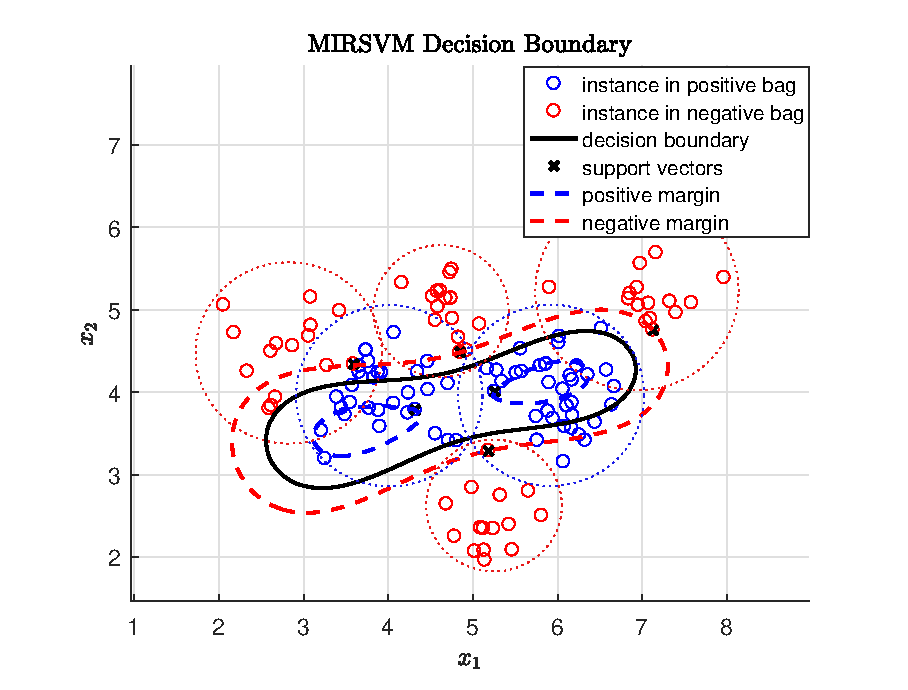
\includegraphics[width=\textwidth]{mirsvm_figure.eps} % first figure itself
    \end{minipage}\hfill
    \begin{minipage}{0.5\textwidth}
        \centering
        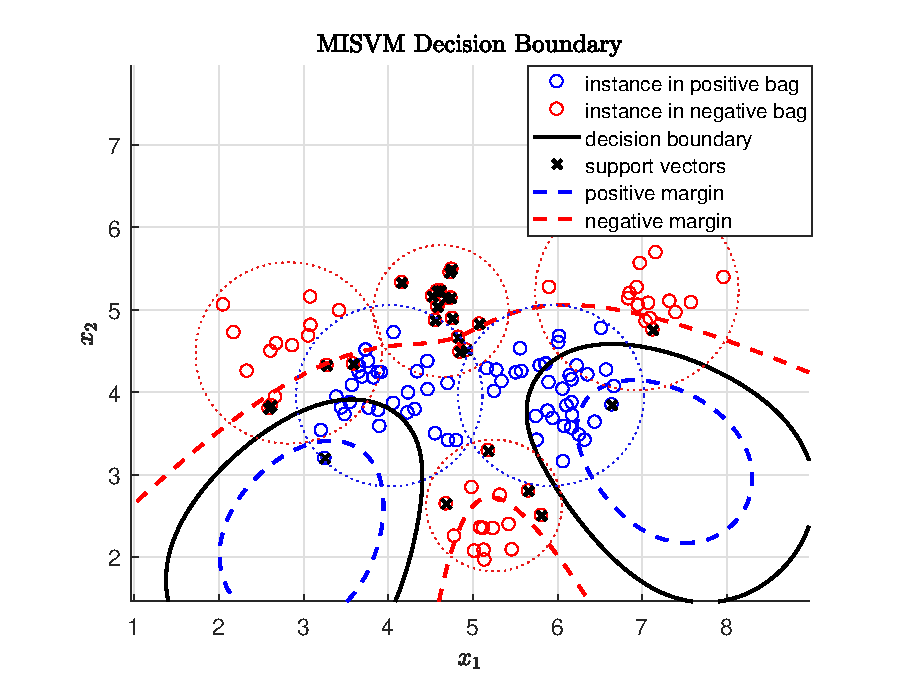
\includegraphics[width=\textwidth]{misvm_figure.eps} % second figure itself
    \end{minipage}
    \caption{Difference between MIRSVM and MISVM on a random $2$-dimensional toy dataset. The instances of this dataset were drawn from the standard normal distribution, with $6$ bags, $4$ of which are negative (red) and $2$ of which are positive (blue), indicated by the red and blue dotted circles. There are a total of $125$ instances, $65$ belonging to the positive bags and $60$ belonging to the negative bags. The decision boundaries (black lines) are shown for each of the algorithms, along with the SVM margin (red and blue dashed lines) and support vectors (black crosses). In this example, both MIRSVM and MISVM were trained using $C = 1000$ and $\sigma = 1.5$. Note the differing number of support vectors produced by the two methods. MIRSVM has $6$, one for each bag, and MISVM has $29$. Also note the smoother representation of the data distribution given by MIRSVM's decision boundary, unlike MISVM whose decision boundary was greatly affected by the larger number of support vectors belonging to the negative class with respect to the only $2$ positive support vectors. }
\end{figure}
This formulation is designed to utilize and select representatives from positive and negative bags, unlike MISVM, which only optimizes over representatives from positive bags, while flattening the negative bag instances. MISVM allows multiple representatives to be chosen from negative bags and limits positive bag-representatives to be one, while MIRSVM allows for balanced bag-representative selection, where each bag is allowed one. MISVM also uses a wrapper technique to initialize the positive bag-representatives by taking the mean vector of the instances within each positive bag. This is an implicit assumption that the instances within the positive bags are all positive, whereas MIRSVM's initialization procedure selects an instance from all bags at random, ensuring no noise is added by any wrapper techniques during initialization and no assumptions are made about the instances. Due to the constraints on the representatives, MIRSVM produces sparser models while MISVM has the freedom to select as many negative support vectors as it needs and restricts the support vectors chosen from positive bags to be one. Figure~\ref{fig:diff} shows the decision boundaries produced by MIRSVM and MISVM to highlight the differences in their solutions. As Figure~\ref{fig:diff} shows, MISVM produces a higher number of support vectors from the negative bags, which greatly influences the final decision boundary in favor of the negative class.

\section{Experiments}\label{sec:experiments}
This section presents the experimental setup and comparison of our contribution, as well as ten other state-of-the-art methods on $15$ different benchmark datasets. First, the experimental setup is described and the state-of-the-art methods are listed. The results for each metric, as well as the statistical analysis, are then presented and analyzed. Finally, the run-time and meta-ranks of each algorithm are shown, and the overall performance of the algorithms across each metric is discussed. The main aim of the experiments is to compare our contribution to other multi-instance support vector machines, state-of-the-art multi-instance learners, and ensemble methods. 

\subsection{Experimental Setup}
Table~\ref{tab:Dataset} presents a summary of the $15$ datasets used throughout the experiments, where the number of attributes, bags, and total number of instances are shown. The datasets were obtained from the Weka\footnote{http://www.cs.waikato.ac.nz/ml/weka}~\citep{Hall2009} and KEEL\footnote{http://sci2s.ugr.es/keel/datasets.php}~\citep{Alca2011} dataset repositories. 

\begin{table}[t!]
\caption{Datasets used for the experiments in~\ref{subsec:results}}
\small
\label{tab:Dataset}
\begin{tabularx}{\textwidth}{l@{\extracolsep{\fill}}ccccc}
\hline\noalign{\smallskip}
Dataset & Attributes & Positive Bags & Negative Bags & Total & Instances \\
\noalign{\smallskip}\hline\noalign{\smallskip}
Suramin 			& 20 	& 7 	& 4 	& 11 	& 2378 	\\
EastWest 			& 24 	& 10 	& 10 	& 20 	& 213 	\\
WestEast 			& 24 	& 10 	& 10 	& 20 	& 213 	\\
Musk1 				& 166 	& 47 	& 45 	& 92 	& 476 	\\
Musk2 				& 166 	& 39 	& 63 	& 102 	& 6598 	\\
Webmining			& 5863	& 17	& 58	& 75	& 2212	\\
TRX 				& 8 	& 25 	& 193 	& 168 	& 26611 \\
Mutagenesis-Atoms 	& 10 	& 125 	& 63 	& 188 	& 1618 	\\
Mutagenesis-Bonds 	& 16 	& 125 	& 63 	& 188 	& 3995 	\\
Mutagenesis-Chains 	& 24 	& 125 	& 63 	& 188 	& 5349 	\\
Tiger 				& 230 	& 100 	& 100 	& 200 	& 1391 	\\
Elephant 			& 230 	& 100 	& 100 	& 200 	& 1220 	\\
Fox 				& 230 	& 100 	& 100 	& 200 	& 1320 	\\
Component			& 22	& 423	& 2707	& 3130	& 36894	\\
Function			& 202	& 443	& 4799	& 5242	& 55536	\\
\noalign{\smallskip}\hline
\end{tabularx}
\end{table}

The experimental environment was designed to test the difference in performance of the proposed method against $10$ state-of-the-art algorithms, contrasting instance-level methods and bag-level methods. Instance-level methods include MIOptimalBall, MIBoost, MISVM, MIDD, and MIWrapper. The bag-level methods include MISMO, SimpleMI, and TLC. The ensemble-based bag-space methods, Bagging and Stacking, were also used. The base algorithms selected for the ensembles Bagging and Stacking were TLC, and TLC and SimpleMI, respectively. These algorithms were chosen because they have shown considerable performance in learning multi-instance models, while also having their frameworks readily available for reproducing their results through MILK, the Multi-Instance Learning Kit\footnote{http://www.cs.waikato.ac.nz/ml/milk}~\citep{Xu2003}, used in conjunction with the Weka framework. Experiments were run in an Intel i7-6700k CPU with 32GB RAM. MIRSVM was implemented in MATLAB while the referenced algorithms are available in the Java implementation of Weka.

Experiments were performed using $k$-fold cross validation, with $k = 10$, in order to evaluate the models' performances and tune hyper-parameters. The data is separated fairly into $10$ equally sized sections where, at every iteration of the cross-validation loop, a section is held out as the test set, while the remainder of the data is used for training. This procedure ensures the model is not optimistically biased towards the full dataset. The tuning of the model during cross-validation includes finding the best penalty parameter, $C$, as well as the best shape parameter for the Gaussian radial basis function kernel, $\sigma$. The best hyper-parameters were chosen from the following $6 \times 6$ possible combination runs, shown in Equations~\eqref{eq:paramC} and~\eqref{eq:paramG}, referred to as~\eqref{eq:hyperparam}. 
\begin{subequations}
\label{eq:hyperparam}
\begin{align}
C \in  & \{0.1, 1, 10, 100, 1000, 10000\} \label{eq:paramC}\\
\sigma \in  & \{0.1, 0.5, 1, 2, 5, 10\} \label{eq:paramG}
\end{align}
\end{subequations}

These parameters were also used for the state-of-the-art SVM methods. This was done in order to keep the experimental environment controlled and ensure fair evaluation of the multi-instance SVM algorithms. The parameters for the referenced algorithms used throughout the experiments were those specified by their authors.

\subsection{Results \& Statistical Analysis}\label{subsec:results}
The classification performance was measured using five metrics: Accuracy~\eqref{eq:accuracy}, Precision~\eqref{eq:precision}, Recall~\eqref{eq:recall}, Cohen's kappa rate~\eqref{eq:kappa}, and Area under ROC curve (AUC)~\eqref{eq:auc}. Accuracy can be misleading when classes are imbalanced, as is the case with the \textit{component} and \textit{function} datasets, which have six and ten times as many negative instances than positive, respectively. Cohen's Kappa Rate and the AUC measures are used as complementary measures in order to evaluate the algorithms comprehensively~\citep{Bendavid2008}. Cohen's kappa rate, shown in Equation~\eqref{eq:kappa}, evaluates classifier merit according to the class distribution and ranges between -1 (full disagreement), 0 (random classification), and 1 (full agreement). The AUC metric highlights the trade-off between the true positive rate, or recall, and the false positive rate, as shown in Equation~\eqref{eq:auc}. The values of the true positive (TP), true negative (TN), false positive (FP), and false negative samples (FN) were first collected for each of the classifiers, then the metrics were computed using the equations shown in~\eqref{eq:metrics} on the $n^\prime$ bags of the test data. The run times of each algorithm are also reported to analyze the usability and speed of each of the algorithms across differently sized datasets. The results for these metrics are shown in Tables~\ref{tab:accResults},~\ref{tab:preResults},~\ref{tab:recResults},~\ref{tab:kappaResults},~\ref{tab:aucResults}, and~\ref{tab:time}.
\begin{subequations}
\label{eq:metrics}
\begin{align}
\text{Accuracy} \tab \tab &\dfrac{TP+TN}{n^\prime} \label{eq:accuracy}\\[1.5pt]
\text{Precision} \tab \tab &\dfrac{TP}{TP+FP} \label{eq:precision}\\[1.5pt]
\text{Recall} \tab \tab &\dfrac{TP}{TP+FN} \label{eq:recall}\\[1.5pt]
\text{Cohen's Kappa Rate} \tab \tab &\dfrac{n^\prime - \dfrac{(TP+FN)*(TP+FP)}{n^\prime}}{1 - \dfrac{(TP+FN)*(TP+FP)}{n^\prime}} \label{eq:kappa}\\[1.5pt]
\text{Area Under ROC Curve} \tab \tab &\frac{1 + \dfrac{TP}{TP+FN} - \dfrac{FP}{FP+TN}}{2} \label{eq:auc}
\end{align}
\end{subequations}

In order to analyze the performances of the multiple models, non-parametric statistical tests are used to validate the experimental results obtained~\citep{Derrac2011,Garcia20102044}. The Iman-Davenport non-parametric test is run to investigate whether significant differences exist among the performance of the algorithms~\citep{Garcia2008} by ranking them over the datasets used, using the Friedman test. The algorithm ranks for each metric in Equations~\eqref{eq:metrics} are presented in the last row of the results tables, and the lowest (best) rank value is typeset in bold. Table~\ref{tab:metarank} contains the ranks and meta-rank of all methods, which helps determine and visualize the best performing algorithms across all datasets and metrics. 

After the Iman-Davenport test indicates significant differences, the Bonferroni-Dunn post-hoc test~\citep{Dunn1961} is then used to find where they occur between algorithms by assuming the classifiers' performances are different by at least some critical value~\citep{Garcia2009}. Below each result table, a figure highlighting the critical distance (in gray), from the best ranking algorithm to the rest, is shown. The algorithms to the right of the critical distance bar perform statistically significantly worse than the control algorithm, MIRSVM. Figures \ref{fig:BonfDunnacc}, \ref{fig:BonfDunnprec}, \ref{fig:BonfDunnrec}, \ref{fig:BonfDunnkappa}, \ref{fig:BonfDunnauc}, \ref{fig:BonfDunnpmeta} show the results of the Bonferroni-Dunn post-hoc procedure over the metrics in~\eqref{eq:metrics}, as well as the meta-rank results in Table~\ref{tab:metarank}.

The Nemenyi, Holm, and Shaffer post-hoc~\citep{Gibbons2011,Holander1999} tests were then run for each of the metrics to compute multiple pairwise comparisons between the proposed algorithm and the state-of-the-art methods, investigating whether statistical differences exist among pairs of algorithms. Tables~\ref{tab:statacc},~\ref{tab:statprec},~\ref{tab:statrec},~\ref{tab:statkappa}, and~\ref{tab:statauc} show the $p$-values for the Nemenyi, Holm, and Shaffer tests for $\alpha = 0.05$.

\subsection{Accuracy}
Table~\ref{tab:accResults} shows the accuracy results of the $11$ algorithms over $15$ multi-instance datasets, along with their average and rank. The results indicate that the bag-based and ensemble learners perform better than the instance-based and wrapper methods. Specifically, MIRSVM achieves the best accuracy over $6$ of the $15$ datasets with a competitive average against the Bagging, Stacking, and TLC algorithms. Note that MIRSVM performs better than MISVM for all datasets, indicating that using representatives from each bag and limiting the number of support-vectors per negative bag improves the classification performance. The instance-level classifiers and wrapper methods, such as MIBoost, MIWrapper, and SimpleMI perform the worst. This behavior emphasizes the importance of not making prior assumptions about the positive bags' distributions. 

Figure~\ref{fig:BonfDunnacc} and Table~\ref{tab:statacc} show the results for the statistical analysis on the accuracy results. The algorithms with ranking higher than $5.51$ (MIRSVM rank + Bonferroni-Dunn critical value), to the right of the grey bar in Figure~\ref{fig:BonfDunnacc}, perform statistically worse than MIRSVM. Table~\ref{tab:statacc} shows the $p$-values of the Nemenyi, Holm, and Shaffer tests. The results from these tests are complement each other. Nemenyi's procedure indicates that MIRSVM performs significantly better than all methods (with $p$-values $< 0.01$), except Bagging, Stacking, TLC, and MISMO. The Nemenyi $p$-values for MIBoost, MIWrapper, and SimpleMI are $= 0$, showing that MIRSVM has significantly better accuracy. However, the stricter Holm and Shaffer tests indicate that significant differences exist between MIRSVM and all other classifiers, highlighting MIRSVM's superior classification accuracy. 

\begin{table}[th!]
\caption{Accuracy}\label{tab:accResults}
\resizebox{\textwidth}{!}{\begin{tabular}{l@{\extracolsep{\fill}}cccccccccccc}
\noalign{\smallskip}\hline\noalign{\smallskip}
Datasets &MIRSVM &MIBoost &MIOptimalBall &MIDD &MIWrapper &MISMO &MISVM &SimpleMI &TLC &Bagging &Stacking \\
\noalign{\smallskip}\hline\noalign{\smallskip}
suramin &0.6000 &0.5000 &0.7250 &0.4250 &0.5000 &0.7250 &0.5000 &0.2308 &0.6923 &0.6750 &\textbf{0.7564} &  \\
eastWest &\textbf{0.8000} &0.5000 &0.7250 &0.6125 &0.5000 &0.7125 &0.6375 &0.5000 &0.5000 &0.6375 &0.4500 &  \\
westEast &0.6500 &0.5000 &0.3750 &0.4500 &0.5000 &\textbf{0.7375} &0.4625 &0.5000 &0.5000 &0.6875 &0.6375 &  \\
musk1 &\textbf{0.9022} &0.5109 &0.7717 &0.8804 &0.5109 &0.7826 &0.8043 &0.5109 &0.8587 &0.8804 &0.8587 &  \\
musk2 &\textbf{0.8146} &0.6139 &0.7723 &0.7228 &0.6139 &0.7030 &0.7129 &0.6139 &0.6238 &0.7129 &0.6733 &  \\
webmining &\textbf{0.8500} &0.8142 &0.7699 &0.8142 &0.8142 &0.8407 &0.6903 &0.8142 &0.8142 &0.7876 &0.8053 &  \\
trx &0.8825 &0.8705 &\textbf{0.9016} &0.8808 &0.8705 &0.8705 &0.8705 &0.8705 &0.8756 &0.8964 &0.8860 &  \\
mutagenesis-atoms &0.7714 &0.6649 &0.6436 &0.7074 &0.6649 &0.6915 &0.6649 &0.6649 &0.7766 &\textbf{0.8032} &0.7606 &  \\
mutagenesis-bonds &0.8252 &0.6649 &0.6915 &0.7713 &0.6649 &0.7979 &0.6649 &0.6649 &0.8351 &\textbf{0.8830} &0.8564 &  \\
mutagenesis-chains &0.8411 &0.6649 &0.6702 &0.7766 &0.6649 &0.8351 &0.6649 &0.6649 &0.8404 &\textbf{0.8457} &0.8351 &  \\
tiger &\textbf{0.7750} &0.5000 &0.5000 &0.7100 &0.5000 &0.7200 &0.7550 &0.5000 &0.6650 &0.7700 &0.7250 &  \\
elephant &0.8300 &0.5000 &0.5000 &0.7900 &0.5000 &0.8100 &0.8000 &0.5000 &0.8000 &\textbf{0.8500} &0.8250 &  \\
fox &\textbf{0.6550} &0.5000 &0.5000 &0.5800 &0.5000 &0.5250 &0.5900 &0.5000 &0.6450 &0.6200 &0.6500 &  \\
component &0.9366 &0.8649 &0.8696 &0.8780 &0.8649 &0.8968 &0.8703 &0.8649 &0.9358 &\textbf{0.9371} &0.9355 &  \\
function &0.9523 &0.9155 &0.9138 &0.9193 &0.9155 &0.9376 &0.9195 &0.9155 &0.9649 &\textbf{0.9655} &0.9647 &  \\
\noalign{\smallskip}\hline\noalign{\smallskip}
Average &\textbf{0.8057} &0.6390 &0.6886 &0.7279 &0.6390 &0.7724 &0.7072 &0.6210 &0.7552 &0.7968 &0.7746 &  \\
Ranks &\textbf{2.4000} &8.8000 &7.2667 &6.0333 &8.8000 &4.8000 &7.0667 &9.0000 &4.7333 &2.7667 &4.3333 &  \\
\noalign{\smallskip}\hline
\end{tabular}}
\centering
\resizebox{0.95\textwidth}{!}{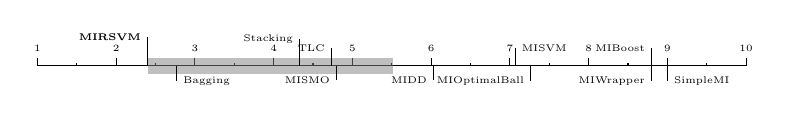
\begin{tikzpicture}
\draw (1,0) -- (10,0);
\foreach \x in {1,2,3,4,5,6,7,8,9,10} {
\draw (\x, 0) -- ++(0,.1) node [above,scale=0.7] {\tiny \x};
\ifthenelse{\x < 10}{\draw (\x+.5, 0) -- ++(0,.03);}{}
}

\coordinate (c0) at (2.4,0);
\coordinate (c1) at (8.8,0);
\coordinate (c2) at (7.2667,0);
\coordinate (c3) at (6.0333,0);
\coordinate (c4) at (8.8,0);
\coordinate (c5) at (4.8,0);
\coordinate (c6) at (7.0667,0);
\coordinate (c7) at (9,0);
\coordinate (c8) at (4.7333,0);
\coordinate (c9) at (2.7667,0);
\coordinate (c10) at (4.3333,0);

\node (l0) at (c0) [above left=.23cm and 0cm, align=right,scale=0.7] {\tiny \textbf{MIRSVM}};
\node (l1) at (c1) [above left=.1cm and 0cm, align=right,scale=0.7] {\tiny MIBoost};
\node (l2) at (c2) [below left=.05cm and 0cm, align=right,scale=0.7] {\tiny MIOptimalBall};
\node (l3) at (c3) [below left=.05cm and 0cm, align=right,scale=0.7] {\tiny MIDD};
\node (l4) at (c4) [below left=.05cm and 0cm, align=right,scale=0.7] {\tiny MIWrapper};
\node (l5) at (c5) [below left=.05cm and 0cm, align=right,scale=0.7] {\tiny MISMO};
\node (l6) at (c6) [above right=.1cm and 0cm, align=right,scale=0.7] {\tiny MISVM};
\node (l7) at (c7) [below right=.05cm and 0cm, align=right,scale=0.7] {\tiny SimpleMI};
\node (l8) at (c8) [above left=.1cm and 0cm, align=right,scale=0.7] {\tiny TLC};
\node (l9) at (c9) [below right=.05cm and 0cm, align=right,scale=0.7] {\tiny Bagging};
\node (l10) at (c10) [above left=.2cm and 0cm, align=right,scale=0.7] {\tiny Stacking};

\fill[fill=gray,fill opacity=0.5] (2.4,-0.1) rectangle (5.5196,0.1);

\foreach \x in {0,1,2,3,4,5,6,7,8,9,10} {
\draw (l\x) -| (c\x);
};
\end{tikzpicture}}
\captionof{figure}{Bonferroni-Dunn test for Accuracy}\label{fig:BonfDunnacc}
\captionof{table}{Nemenyi, Holm, and Shaffer tests for Accuracy}\label{tab:statacc}
\scriptsize
\begin{tabularx}{\textwidth}{lcccccccccc}\noalign{\smallskip}\hline\noalign{\smallskip}
MIRSVM vs. & MIBoost & MIOptimalBall & MIDD & MIWrapper & MISMO & MISVM & SimpleMI & TLC & Bagging & Stacking\\
\noalign{\smallskip}\hline\noalign{\smallskip}
Nemenyi $p$-value & 0.00000 & 0.00006 & 0.00270 & 0.00000 & 0.04751 & 0.00012 & 0.00000 & 0.05402 & 0.76207 & 0.11040\\
Holm $p$-value & 0.00093 & 0.00102 & 0.00139 & 0.00094 & 0.00185 & 0.00104 & 0.00091 & 0.00192 & 0.00833 & 0.00238\\
Shaffer $p$-value & 0.00111 & 0.00111 & 0.00139 & 0.00111 & 0.00185 & 0.00111 & 0.00091 & 0.00192 & 0.00833 & 0.00238\\
\noalign{\smallskip}\hline\noalign{\smallskip}
\end{tabularx}
\end{table}
\newpage
\subsection{Precision \& Recall}
Precision and recall are metrics that must be evaluated together in order to observe their behavior simultaneously, since they are both metrics used to measure relevance. Tables~\ref{tab:preResults} and~\ref{tab:recResults} show the precision and recall results obtained by each algorithm. The precision and recall results for MIWrapper and SimpleMI indicate that they are unstable classifiers, exhibiting extreme variance in behavior, making them unsuitable for real-world applications. It is also interesting to analyze the performance on the mutagenesis datasets, where MISVM, MIBoost, MIWrapper, and SimpleMI predict all bags as negative. Additionally, while MISMO obtains unbiased results on these datasets, MIRSVM significantly outperforms it over both precision and recall.  

Figure~\ref{fig:BonfDunnprec} shows that there are no statistically significant differences between the precision results obtained by all algorithms, except SimpleMI; and Figure~\ref{fig:BonfDunnrec} shows none over all. It is worth noting that MIRSVM outperforms both ensemble methods according to recall, despite them exhibiting relatively good accuracy and precision. This indicates that they are strongly conservative towards predicting positive bags. The Holm and Shaffer tests indicate that significant differences exist between MIRSVM and the state-of-the-art, with the exception of SimpleMI. 

\begin{table}[t!]
\caption{Precision}\label{tab:preResults}
\resizebox{\textwidth}{!}{\begin{tabular}{l@{\extracolsep{\fill}}cccccccccccc}
\noalign{\smallskip}\hline\noalign{\smallskip}
Datasets &MIRSVM &MIBoost &MIOptimalBall &MIDD &MIWrapper &MISMO &MISVM &SimpleMI &TLC &Bagging &Stacking \\
\noalign{\smallskip}\hline\noalign{\smallskip}
suramin &0.6385 &\textbf{1.0000} &\textbf{1.0000} &0.2857 &\textbf{1.0000} &\textbf{1.0000} &0.5000 &0.0000 &0.6667 &0.7333 &0.7116 &  \\
eastWest &0.7143 &0.5000 &\textbf{0.8750} &0.5882 &0.5000 &0.7429 &0.8667 &0.5000 &0.5000 &0.6667 &0.4444 &  \\
westEast &0.6300 &0.5000 &0.2727 &0.4600 &0.5000 &\textbf{0.6939} &0.3846 &0.5000 &0.5000 &0.6364 &0.6038 &  \\
musk1 &0.8519 &\textbf{1.0000} &0.9286 &0.9048 &\textbf{1.0000} &0.8049 &0.8857 &\textbf{1.0000} &0.8478 &0.9250 &0.8478 &  \\
musk2 &0.7167 &0.6139 &\textbf{0.7826} &0.7576 &0.6139 &0.7424 &0.7538 &0.6139 &0.7400 &0.7797 &0.7164 &  \\
webmining &0.7500 &0.8142 &0.8173 &0.8142 &0.8142 &0.8936 &\textbf{1.0000} &0.8142 &0.8817 &0.8469 &0.8500 &  \\
trx &0.6500 &0.8705 &\textbf{0.9306} &0.9191 &0.8705 &0.8705 &0.8705 &0.8705 &0.9138 &0.8936 &0.9011 &  \\
mutagenesis-atoms &0.7872 &\textbf{1.0000} &0.4630 &0.6111 &\textbf{1.0000} &0.5439 &\textbf{1.0000} &\textbf{1.0000} &0.7059 &0.7321 &0.6667 &  \\
mutagenesis-bonds &0.8468 &\textbf{1.0000} &0.5385 &0.7500 &\textbf{1.0000} &0.6812 &\textbf{1.0000} &\textbf{1.0000} &0.7857 &0.8596 &0.8333 &  \\
mutagenesis-chains &0.8571 &\textbf{1.0000} &0.5091 &0.7059 &\textbf{1.0000} &0.7759 &\textbf{1.0000} &\textbf{1.0000} &0.7705 &0.7742 &0.7581 &  \\
tiger &0.7365 &0.5000 &0.5000 &0.6944 &0.5000 &0.7444 &0.7802 &0.5000 &0.6514 &\textbf{0.7935} &0.7320 &  \\
elephant &0.8576 &0.5000 &0.5000 &0.7959 &0.5000 &0.8444 &0.7679 &0.5000 &0.8000 &\textbf{0.8804} &0.8283 &  \\
fox &0.6040 &0.5000 &0.5000 &0.5833 &0.5000 &0.5287 &0.6216 &0.5000 &\textbf{0.6747} &0.6304 &0.6705 &  \\
component &\textbf{0.9866} &0.8649 &0.8778 &0.8902 &0.8649 &0.8958 &0.8696 &0.8649 &0.9462 &0.9431 &0.9449 &  \\
function &0.8459 &0.9155 &0.9202 &0.9317 &0.9155 &0.9376 &0.9197 &0.9155 &\textbf{0.9729} &0.9720 &0.9726 &  \\
\noalign{\smallskip}\hline\noalign{\smallskip}
Average &0.7649 &0.7719 &0.6944 &0.7128 &0.7719 &0.7800 &\textbf{0.8147} &0.7053 &0.7572 &0.8045 &0.7654 &  \\
Ranks &6.0667 &6.7333 &6.7333 &6.7667 &6.7333 &5.3667 &5.1000 &7.3000 &5.5000 &\textbf{3.9333} &5.7667 &  \\
\noalign{\smallskip}\hline
\end{tabular}}
\centering
\resizebox{0.95\textwidth}{!}{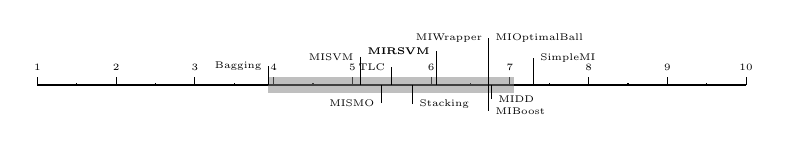
\begin{tikzpicture}
\draw (1,0) -- (10,0);
\foreach \x in {1,2,3,4,5,6,7,8,9,10} {
\draw (\x, 0) -- ++(0,.1) node [above,scale=0.7] {\tiny \x};
\ifthenelse{\x < 10}{\draw (\x+.5, 0) -- ++(0,.03);}{}
}

\coordinate (c0) at (6.0667,0);
\coordinate (c1) at (6.7333,0);
\coordinate (c2) at (6.7333,0);
\coordinate (c3) at (6.7667,0);
\coordinate (c4) at (6.7333,0);
\coordinate (c5) at (5.3667,0);
\coordinate (c6) at (5.1,0);
\coordinate (c7) at (7.3,0);
\coordinate (c8) at (5.5,0);
\coordinate (c9) at (3.9333,0);
\coordinate (c10) at (5.7667,0);

\node (l0) at (c0) [above left=.3cm and 0cm, align=right,scale=0.7] {\tiny \textbf{MIRSVM}};
\node (l1) at (c1) [below right=.2cm and 0cm, align=right,scale=0.7] {\tiny MIBoost};
\node (l2) at (c2) [above right=.45cm and 0cm, align=right,scale=0.7] {\tiny MIOptimalBall};
\node (l3) at (c3) [below right=.05cm and 0cm, align=right,scale=0.7] {\tiny MIDD};
\node (l4) at (c4) [above left=.45cm and 0cm, align=right,scale=0.7] {\tiny MIWrapper};
\node (l5) at (c5) [below left=.1cm and 0cm, align=right,scale=0.7] {\tiny MISMO};
\node (l6) at (c6) [above left=.23cm and 0cm, align=right,scale=0.7] {\tiny MISVM};
\node (l7) at (c7) [above right=.2cm and 0cm, align=right,scale=0.7] {\tiny SimpleMI};
\node (l8) at (c8) [above left=.1cm and 0cm, align=right,scale=0.7] {\tiny TLC};
\node (l9) at (c9) [above left=.1cm and 0cm, align=right,scale=0.7] {\tiny Bagging};
\node (l10) at (c10) [below right=.1cm and 0cm, align=right,scale=0.7] {\tiny Stacking};

\fill[fill=gray,fill opacity=0.5] (3.9333,-0.1) rectangle (7.0529,0.1);

\foreach \x in {0,1,2,3,4,5,6,7,8,9,10} {
\draw (l\x) -| (c\x);
};
\end{tikzpicture}}
\captionof{figure}{Bonferroni-Dunn test for Precision}\label{fig:BonfDunnprec}
\captionof{table}{Nemenyi, Holm, and Shaffer tests for Precision}\label{tab:statprec}
\scriptsize
\begin{tabularx}{\textwidth}{lcccccccccc}\noalign{\smallskip}\hline\noalign{\smallskip}
MIRSVM vs. & MIBoost & MIOptimalBall & MIDD & MIWrapper & MISMO & MISVM & SimpleMI & TLC & Bagging & Stacking\\
\noalign{\smallskip}\hline\noalign{\smallskip}
Nemenyi $p$-value & 0.58199 & 0.58199 & 0.56326 & 0.58199 & 0.56326 & 0.42475 & 0.30849 & 0.63985 & 0.07815 & 0.80435\\
Holm $p$-value & 0.00263 & 0.00250 & 0.00217 & 0.00278 & 0.00227 & 0.00185 & 0.00156 & 0.00294 & 0.00102 & 0.00500\\
Shaffer $p$-value & 0.00263 & 0.00250 & 0.00217 & 0.00278 & 0.00227 & 0.00185 & 0.00156 & 0.00294 & 0.00102 & 0.00500\\
\noalign{\smallskip}\hline\noalign{\smallskip}
\end{tabularx}
\end{table}
\begin{table}[h!]
\caption{Recall}\label{tab:recResults}
\resizebox{\textwidth}{!}{\begin{tabular}{l@{\extracolsep{\fill}}cccccccccccc}
\noalign{\smallskip}\hline\noalign{\smallskip}
Datasets &MIRSVM &MIBoost &MIOptimalBall &MIDD &MIWrapper &MISMO &MISVM &SimpleMI &TLC &Bagging &Stacking \\
\noalign{\smallskip}\hline\noalign{\smallskip}
suramin &\textbf{1.0000} &0.0000 &0.4500 &0.1000 &0.0000 &0.4500 &0.5000 &0.0000 &0.6667 &0.5500 &0.9125 &  \\
eastWest &\textbf{1.0000} &0.7000 &0.5250 &0.7500 &0.7000 &0.6500 &0.3250 &\textbf{1.0000} &0.5000 &0.5500 &0.4000 &  \\
westEast &0.9000 &0.9000 &0.1500 &0.5750 &0.9000 &0.8500 &0.1250 &\textbf{1.0000} &0.5000 &0.8750 &0.8000 &  \\
musk1 &\textbf{0.9787} &0.0000 &0.5778 &0.8444 &0.0000 &0.7333 &0.6889 &0.0000 &0.8667 &0.8222 &0.8667 &  \\
musk2 &0.9250 &\textbf{1.0000} &0.8710 &0.8065 &\textbf{1.0000} &0.7903 &0.7903 &\textbf{1.0000} &0.5968 &0.7419 &0.7742 &  \\
webmining &0.2857 &\textbf{1.0000} &0.9239 &\textbf{1.0000} &\textbf{1.0000} &0.9130 &0.6196 &\textbf{1.0000} &0.8913 &0.9022 &0.9239 &  \\
trx &0.4833 &\textbf{1.0000} &0.9583 &0.9464 &\textbf{1.0000} &\textbf{1.0000} &\textbf{1.0000} &\textbf{1.0000} &0.9464 &\textbf{1.0000} &0.9762 &  \\
mutagenesis-atoms &\textbf{0.8880} &0.0000 &0.3968 &0.3492 &0.0000 &0.4921 &0.0000 &0.0000 &0.5714 &0.6508 &0.5714 &  \\
mutagenesis-bonds &\textbf{0.8960} &0.0000 &0.5556 &0.4762 &0.0000 &0.7460 &0.0000 &0.0000 &0.6984 &0.7778 &0.7143 &  \\
mutagenesis-chains &\textbf{0.9120} &0.0000 &0.4444 &0.5714 &0.0000 &0.7143 &0.0000 &0.0000 &0.7460 &0.7619 &0.7460 &  \\
tiger &0.8700 &0.5000 &\textbf{1.0000} &0.7500 &0.5000 &0.6700 &0.7100 &\textbf{1.0000} &0.7100 &0.7300 &0.7100 &  \\
elephant &0.9100 &0.6000 &\textbf{1.0000} &0.7800 &0.6000 &0.7600 &0.8600 &\textbf{1.0000} &0.8000 &0.8100 &0.8200 &  \\
fox &0.9000 &0.7000 &\textbf{1.0000} &0.5600 &0.7000 &0.4600 &0.4600 &\textbf{1.0000} &0.5600 &0.5800 &0.5900 &  \\
component &0.5839 &\textbf{1.0000} &0.9867 &0.9797 &\textbf{1.0000} &0.9967 &\textbf{1.0000} &\textbf{1.0000} &0.9815 &0.9867 &0.9826 &  \\
function &0.5327 &\textbf{1.0000} &0.9919 &0.9840 &\textbf{1.0000} &0.9983 &0.9994 &\textbf{1.0000} &0.9892 &0.9908 &0.9894 &  \\
\noalign{\smallskip}\hline\noalign{\smallskip}
Average &\textbf{0.8044} &0.5600 &0.7221 &0.6982 &0.5600 &0.7483 &0.5385 &0.6667 &0.7350 &0.7820 &0.7851 &  \\
Ranks &\textbf{4.4333} &6.2667 &5.8000 &6.7667 &6.2667 &6.2667 &7.4333 &4.5333 &7.0333 &5.3333 &5.8667 &  \\
\noalign{\smallskip}\hline
\end{tabular}}
\resizebox{0.95\textwidth}{!}{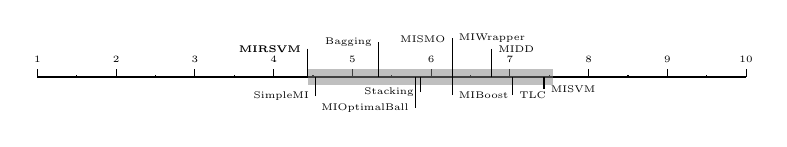
\begin{tikzpicture}
\draw (1,0) -- (10,0);
\foreach \x in {1,2,3,4,5,6,7,8,9,10} {
\draw (\x, 0) -- ++(0,.1) node [above,scale=0.7] {\tiny \x};
\ifthenelse{\x < 10}{\draw (\x+.5, 0) -- ++(0,.03);}{}
}

\coordinate (c0) at (4.4333,0);
\coordinate (c1) at (6.2667,0);
\coordinate (c2) at (5.8,0);
\coordinate (c3) at (6.7667,0);
\coordinate (c4) at (6.2667,0);
\coordinate (c5) at (6.2667,0);
\coordinate (c6) at (7.4333,0);
\coordinate (c7) at (4.5333,0);
\coordinate (c8) at (7.0333,0);
\coordinate (c9) at (5.3333,0);
\coordinate (c10) at (5.8667,0);

\node (l0) at (c0) [above left=.23cm and 0cm, align=right,scale=0.7] {\tiny \textbf{MIRSVM}};
\node (l1) at (c1) [below right=.1cm and 0cm, align=right,scale=0.7] {\tiny MIBoost};
\node (l2) at (c2) [below left=.25cm and 0cm, align=right,scale=0.7] {\tiny MIOptimalBall};
\node (l3) at (c3) [above right=.23cm and 0cm, align=right,scale=0.7] {\tiny MIDD};
\node (l4) at (c4) [above right=.35cm and 0cm, align=right,scale=0.7] {\tiny MIWrapper};
\node (l5) at (c5) [above left=.35cm and 0cm, align=right,scale=0.7] {\tiny MISMO};
\node (l6) at (c6) [below right=.025cm and 0cm, align=right,scale=0.7] {\tiny MISVM};
\node (l7) at (c7) [below left=.1cm and 0cm, align=right,scale=0.7] {\tiny SimpleMI};
\node (l8) at (c8) [below right=.1cm and 0cm, align=right,scale=0.7] {\tiny TLC};
\node (l9) at (c9) [above left=.3cm and 0cm, align=right,scale=0.7] {\tiny Bagging};
\node (l10) at (c10) [below left=.05cm and 0cm, align=right,scale=0.7] {\tiny Stacking};

\fill[fill=gray,fill opacity=0.5] (4.4333,-0.1) rectangle (7.5529,0.1);

\foreach \x in {0,1,2,3,4,5,6,7,8,9,10} {
\draw (l\x) -| (c\x);
};
\end{tikzpicture}}
\captionof{figure}{Bonferroni-Dunn test for Recall}\label{fig:BonfDunnrec}
\captionof{table}{Nemenyi, Holm, and Shaffer tests for Recall}\label{tab:statrec}
\scriptsize
\begin{tabularx}{\textwidth}{lcccccccccc}\noalign{\smallskip}\hline\noalign{\smallskip}
MIRSVM vs. & MIBoost & MIOptimalBall & MIDD & MIWrapper & MISMO & MISVM & SimpleMI & TLC & Bagging & Stacking\\
\noalign{\smallskip}\hline\noalign{\smallskip}
Nemenyi $p$-value & 0.13007 & 0.25911 & 0.05402 & 0.13007 & 0.13007 & 0.01324 & 0.93419 & 0.03180 & 0.45739 & 0.23660\\
Holm $p$-value & 0.00104 & 0.00135 & 0.00098 & 0.00106 & 0.00109 & 0.00090 & 0.01000 & 0.00094 & 0.00208 & 0.00132\\
Shaffer $p$-value & 0.00104 & 0.00135 & 0.00098 & 0.00106 & 0.00109 & 0.00090 & 0.01000 & 0.00094 & 0.00208 & 0.00132\\
\noalign{\smallskip}\hline\noalign{\smallskip}
\end{tabularx}
\end{table}

\subsection{Cohen's Kappa Rate}
Table~\ref{tab:kappaResults} shows the Cohen's Kappa rate results obtained by the algorithms. These results support the accuracy achieved by the algorithms, in the sense that the instance-based and wrapper methods perform worse than bag-based and ensemble learners. Specifically, MIRSVM achieves the best kappa rate over $7$ of the $15$ datasets with a competitive average against the Bagging, Stacking, SMO, and TLC algorithms. MIRSVM's kappa values all fall within the range ($0.5$-$1$], indicating that its merit as a classifier agrees with the class distribution and is not random. Note that SimpleMI, MIOptimalBall, MIDD, MISVM, and Stacking contain some negative kappa values, indicating performance worse than the default-hypothesis. MIBoost and MIWrapper are shown to randomly classify all $15$ datasets. 

Figure~\ref{fig:BonfDunnkappa} and Table~\ref{tab:statkappa} show the results of the statistical analysis on the Cohen's Kappa Rate results. Nemenyi's procedure reflects results similar to the $p$-values obtained from the accuracy results, where MIRSVM performs significantly better than MIOptimalBall, MIDD, MISVM, MIWrapper, MIBoost, and SimpleMI, having $p$-values $< 0.01$. The Holm and Shaffer procedures indicate that significant differences exist among all algorithms results, supporting MIRSVM's performance as a competitive classifier.

\begin{table}[t!]
\caption{Cohen's Kappa Rate}\label{tab:kappaResults}
\resizebox{\textwidth}{!}{\begin{tabular}{lcccccccccccc}
\noalign{\smallskip}\hline\noalign{\smallskip}
Datasets &MIRSVM &MIBoost &MIOptimalBall &MIDD &MIWrapper &MISMO &MISVM &SimpleMI &TLC &Bagging &Stacking \\
\noalign{\smallskip}\hline\noalign{\smallskip}
suramin &\textbf{0.6320} &0.0000 &0.4500 &-0.1500 &0.0000 &0.4500 &0.0000 &-0.5854 &0.3810 &0.3500 &0.5121 &  \\
eastWest &\textbf{0.6000} &0.0000 &0.4500 &0.2250 &0.0000 &0.4250 &0.2750 &0.0000 &0.0000 &0.2750 &-0.1000 &  \\
westEast &0.3500 &0.0000 &-0.2500 &-0.1000 &0.0000 &\textbf{0.4750} &-0.0750 &0.0000 &0.0000 &0.3750 &0.2750 &  \\
musk1 &\textbf{0.8036} &0.0000 &0.5396 &0.7604 &0.0000 &0.5642 &0.6067 &0.0000 &0.7174 &0.7602 &0.7174 &  \\
musk2 &\textbf{0.6263} &0.0000 &0.5031 &0.4039 &0.0000 &0.3613 &0.3856 &0.0000 &0.2492 &0.4029 &0.2940 &  \\
webmining &0.3468 &0.0000 &0.0246 &0.0000 &0.0000 &\textbf{0.4535} &0.3771 &0.0000 &0.3744 &0.2112 &0.2458 &  \\
trx &0.4542 &0.0000 &\textbf{0.5228} &0.4224 &0.0000 &0.0000 &0.0000 &0.0000 &0.3858 &0.3032 &0.3364 &  \\
mutagenesis-atoms &0.5395 &0.0000 &0.1709 &0.2654 &0.0000 &0.2909 &0.0000 &0.0000 &0.4738 &\textbf{0.5458} &0.4431 &  \\
mutagenesis-bonds &0.5699 &0.0000 &0.3131 &0.4356 &0.0000 &0.5569 &0.0000 &0.0000 &0.6195 &\textbf{0.7310} &0.6659 &  \\
mutagenesis-chains &0.6303 &0.0000 &0.2359 &0.4738 &0.0000 &0.6225 &0.0000 &0.0000 &0.6391 &\textbf{0.6525} &0.6285 &  \\
tiger &\textbf{0.5500} &0.0000 &0.0000 &0.4200 &0.0000 &0.4400 &0.5100 &0.0000 &0.3300 &0.5400 &0.4500 &  \\
elephant &\textbf{0.7000} &0.0000 &0.0000 &0.5800 &0.0000 &0.6200 &0.6000 &0.0000 &0.6000 &\textbf{0.7000} &0.6500 &  \\
fox &\textbf{0.3100} &0.0000 &0.0000 &0.1600 &0.0000 &0.0500 &0.1800 &0.0000 &0.2900 &0.2400 &0.3000 &  \\
component &0.6644 &0.0000 &0.1613 &0.2836 &0.0000 &0.3656 &0.0675 &0.0000 &\textbf{0.6945} &0.6924 &0.6906 &  \\
function &0.6292 &0.0000 &0.0966 &0.2801 &0.0000 &0.4083 &0.0933 &0.0000 &0.7529 &\textbf{0.7534} &0.7507 &  \\
\noalign{\smallskip}\hline\noalign{\smallskip}
Average &\textbf{0.5604} &0.0000 &0.2145 &0.2973 &0.0000 &0.4055 &0.2013 &-0.0390 &0.4338 &0.5022 &0.4573 &  \\
Ranks &\textbf{2.2333} &9.2333 &6.5333 &6.1667 &9.2333 &4.7667 &6.7667 &9.4333 &4.4000 &3.0000 &4.2333 &  \\
\noalign{\smallskip}\hline\noalign{\smallskip}
\end{tabular}}
\centering
\resizebox{0.95\textwidth}{!}{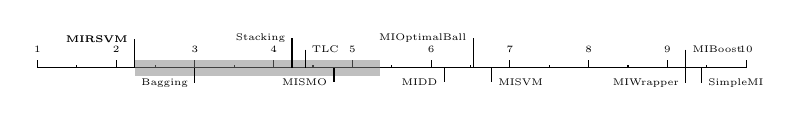
\begin{tikzpicture}
\draw (1,0) -- (10,0);
\foreach \x in {1,2,3,4,5,6,7,8,9,10} {
\draw (\x, 0) -- ++(0,.1) node [above,scale=0.7] {\tiny \x};
\ifthenelse{\x < 10}{\draw (\x+.5, 0) -- ++(0,.03);}{}
}

\coordinate (c0) at (2.2333,0);
\coordinate (c1) at (9.2333,0);
\coordinate (c2) at (6.5333,0);
\coordinate (c3) at (6.1667,0);
\coordinate (c4) at (9.2333,0);
\coordinate (c5) at (4.7667,0);
\coordinate (c6) at (6.7667,0);
\coordinate (c7) at (9.4333,0);
\coordinate (c8) at (4.4,0);
\coordinate (c9) at (3,0);
\coordinate (c10) at (4.2333,0);

\node (l0) at (c0) [above left=.23cm and 0cm, align=right,scale=0.7] {\tiny \textbf{MIRSVM}};
\node (l1) at (c1) [above right=.1cm and 0cm, align=right,scale=0.7] {\tiny MIBoost};
\node (l2) at (c2) [above left=.23cm and 0cm, align=right,scale=0.7] {\tiny MIOptimalBall};
\node (l3) at (c3) [below left=.05cm and 0cm, align=right,scale=0.7] {\tiny MIDD};
\node (l4) at (c4) [below left=.05cm and 0cm, align=right,scale=0.7] {\tiny MIWrapper};
\node (l5) at (c5) [below left=.05cm and 0cm, align=right,scale=0.7] {\tiny MISMO};
\node (l6) at (c6) [below right=.05cm and 0cm, align=right,scale=0.7] {\tiny MISVM};
\node (l7) at (c7) [below right=.05cm and 0cm, align=right,scale=0.7] {\tiny SimpleMI};
\node (l8) at (c8) [above right=.1cm and 0cm, align=right,scale=0.7] {\tiny TLC};
\node (l9) at (c9) [below left=.05cm and 0cm, align=right,scale=0.7] {\tiny Bagging};
\node (l10) at (c10) [above left=.23cm and 0cm, align=right,scale=0.7] {\tiny Stacking};

\fill[fill=gray,fill opacity=0.5] (2.2333,-0.1) rectangle (5.3529,0.1);

\foreach \x in {0,1,2,3,4,5,6,7,8,9,10} {
\draw (l\x) -| (c\x);
};
\end{tikzpicture}}
\captionof{figure}{Bonferroni-Dunn test for Cohen's Kappa rate}\label{fig:BonfDunnkappa}
\vspace{0.5cm}
\captionof{table}{Nemenyi, Holm, and Shaffer tests for Cohen's Kappa rate}\label{tab:statkappa}
\scriptsize
\begin{tabularx}{\textwidth}{lcccccccccc}\noalign{\smallskip}\hline\noalign{\smallskip}
MIRSVM vs. & MIBoost & MIOptimalBall & MIDD & MIWrapper & MISMO & MISVM & SimpleMI & TLC & Bagging & Stacking\\
\noalign{\smallskip}\hline\noalign{\smallskip}
Nemenyi $p$-value & 0.00000 & 0.00105 & 0.00353 & 0.00000 & 0.03180 & 0.00018 & 0.00000 & 0.03899 & 0.49139 & 0.13720\\
Holm $p$-value & 0.00091 & 0.00128 & 0.00143 & 0.00093 & 0.00200 & 0.00119 & 0.00094 & 0.00208 & 0.00556 & 0.00263\\
Shaffer $p$-value & 0.00091 & 0.00135 & 0.00143 & 0.00111 & 0.00200 & 0.00135 & 0.00111 & 0.00208 & 0.00556 & 0.00263\\
\noalign{\smallskip}\hline\noalign{\smallskip}
\end{tabularx}
\end{table}
\bigskip
\begin{table}[H]
\caption{AUC}\label{tab:aucResults}
\resizebox{\textwidth}{!}{\begin{tabular}{lcccccccccccc}
\hline\noalign{\smallskip}
Datasets &MIRSVM &MIBoost &MIOptimalBall &MIDD &MIWrapper &MISMO &MISVM &SimpleMI &TLC &Bagging &Stacking \\
\hline\noalign{\smallskip}
suramin &0.5000 &0.5000 &\textbf{0.7250} &0.4250 &0.5000 &\textbf{0.7250} &0.5000 &0.2143 &0.6905 &0.6750 &0.6811 &  \\
eastWest &\textbf{0.8000} &0.5000 &0.7250 &0.6125 &0.5000 &0.7125 &0.6375 &0.5000 &0.5000 &0.6375 &0.4500 &  \\
westEast &0.6500 &0.5000 &0.3750 &0.4500 &0.5000 &\textbf{0.7375} &0.4625 &0.5000 &0.5000 &0.6875 &0.6375 &  \\
musk1 &\textbf{0.9005} &0.5000 &0.7676 &0.8797 &0.5000 &0.7816 &0.8019 &0.5000 &0.8589 &0.8792 &0.8589 &  \\
musk2 &\textbf{0.8351} &0.5000 &0.7432 &0.6981 &0.5000 &0.6772 &0.6900 &0.5000 &0.6317 &0.7043 &0.6435 &  \\
webmining &0.6320 &0.5000 &0.5096 &0.5000 &0.5000 &0.7184 &\textbf{0.8098} &0.5000 &0.6837 &0.5939 &0.6048 &  \\
trx &0.7243 &0.5000 &\textbf{0.7392} &0.6932 &0.5000 &0.5000 &0.5000 &0.5000 &0.6732 &0.6000 &0.6281 &  \\
mutagenesis-atoms &0.7106 &0.5000 &0.5824 &0.6186 &0.5000 &0.6420 &0.5000 &0.5000 &0.7257 &\textbf{0.7654} &0.7137 &  \\
mutagenesis-bonds &0.7856 &0.5000 &0.6578 &0.6981 &0.5000 &0.7850 &0.5000 &0.5000 &0.8012 &\textbf{0.8569} &0.8211 &  \\
mutagenesis-chains &\textbf{0.8252} &0.5000 &0.6142 &0.7257 &0.5000 &0.8051 &0.5000 &0.5000 &0.8170 &0.8250 &0.8130 &  \\
tiger &\textbf{0.7750} &0.5000 &0.5000 &0.7100 &0.5000 &0.7200 &0.7550 &0.5000 &0.6650 &0.7700 &0.7250 &  \\
elephant &0.8200 &0.5000 &0.5000 &0.7900 &0.5000 &0.8100 &0.8000 &0.5000 &0.8000 &\textbf{0.8500} &0.8250 &  \\
fox &\textbf{0.6550} &0.5000 &0.5000 &0.5800 &0.5000 &0.5250 &0.5900 &0.5000 &0.6450 &0.6200 &0.6500 &  \\
component &0.7855 &0.5000 &0.5536 &0.6033 &0.5000 &0.6272 &0.5201 &0.5000 &\textbf{0.8123} &0.8030 &0.8081 &  \\
function &0.7563 &0.5000 &0.5298 &0.6015 &0.5000 &0.6391 &0.5268 &0.5000 &\textbf{0.8456} &0.8408 &0.8434 &  \\
\hline\noalign{\smallskip}\noalign{\smallskip}
Average &\textbf{0.7437} &0.5000 &0.6015 &0.6390 &0.5000 &0.6937 &0.6062 &0.4810 &0.7100 &0.7406 &0.7135 &  \\
Ranks &\textbf{2.7667} &9.2000 &6.4000 &6.2333 &9.2000 &4.7000 &6.6667 &9.4333 &4.2000 &3.1000 &4.1000 &  \\
\hline\noalign{\smallskip}
\end{tabular}}
\centering
\resizebox{0.9\textwidth}{!}{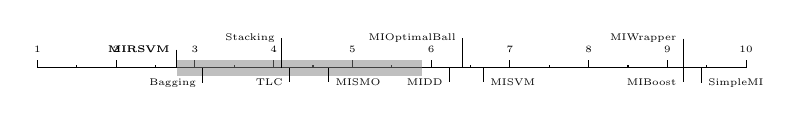
\begin{tikzpicture}
\draw (1,0) -- (10,0);
\foreach \x in {1,2,3,4,5,6,7,8,9,10} {
\draw (\x, 0) -- ++(0,.1) node [above,scale=0.7] {\tiny \x};
\ifthenelse{\x < 10}{\draw (\x+.5, 0) -- ++(0,.03);}{}
}

\coordinate (c0) at (2.7667,0);
\coordinate (c1) at (9.2,0);
\coordinate (c2) at (6.4,0);
\coordinate (c3) at (6.2333,0);
\coordinate (c4) at (9.2,0);
\coordinate (c5) at (4.7,0);
\coordinate (c6) at (6.6667,0);
\coordinate (c7) at (9.4333,0);
\coordinate (c8) at (4.2,0);
\coordinate (c9) at (3.1,0);
\coordinate (c10) at (4.1,0);

\node (l0) at (c0) [above left=.1cm and 0cm, align=right,scale=0.7] {\tiny \textbf{MIRSVM}};
\node (l1) at (c1) [below left=.05cm and 0cm, align=right,scale=0.7] {\tiny MIBoost};
\node (l2) at (c2) [above left=.23cm and 0cm, align=right,scale=0.7] {\tiny MIOptimalBall};
\node (l3) at (c3) [below left=.05cm and 0cm, align=right,scale=0.7] {\tiny MIDD};
\node (l4) at (c4) [above left=.23cm and 0cm, align=right,scale=0.7] {\tiny MIWrapper};
\node (l5) at (c5) [below right=.05cm and 0cm, align=right,scale=0.7] {\tiny MISMO};
\node (l6) at (c6) [below right=.05cm and 0cm, align=right,scale=0.7] {\tiny MISVM};
\node (l7) at (c7) [below right=.05cm and 0cm, align=right,scale=0.7] {\tiny SimpleMI};
\node (l8) at (c8) [below left=.05cm and 0cm, align=right,scale=0.7] {\tiny TLC};
\node (l9) at (c9) [below left=.05cm and 0cm, align=right,scale=0.7] {\tiny Bagging};
\node (l10) at (c10) [above left=.23cm and 0cm, align=right,scale=0.7] {\tiny Stacking};

\fill[fill=gray,fill opacity=0.5] (2.7667,-0.1) rectangle (5.8863,0.1);

\foreach \x in {0,1,2,3,4,5,6,7,8,9,10} {
\draw (l\x) -| (c\x);
};
\end{tikzpicture}}
\captionof{figure}{Bonferroni-Dunn test for AUC}\label{fig:BonfDunnauc}
\vspace{0.5cm}
\captionof{table}{Nemenyi, Holm, and Shaffer tests for AUC}\label{tab:statauc}
\scriptsize
\begin{tabularx}{\textwidth}{lcccccccccc}\noalign{\smallskip}\hline\noalign{\smallskip}
MIRSVM vs. & MIBoost & MIOptimalBall & MIDD & MIWrapper & MISMO & MISVM & SimpleMI & TLC & Bagging & Stacking\\
\noalign{\smallskip}\hline\noalign{\smallskip}
Nemenyi $p$-value & 0.00000 & 0.00270 & 0.00420 & 0.00000 & 0.11040 & 0.00128 & 0.00000 & 0.23660 & 0.78313 & 0.27091\\
Holm $p$-value & 0.00093 & 0.00128 & 0.00135 & 0.00094 & 0.00278 & 0.00125 & 0.00091 & 0.00357 & 0.00714 & 0.00385\\
Shaffer $p$-value & 0.00111 & 0.00135 & 0.00135 & 0.00111 & 0.00278 & 0.00135 & 0.00091 & 0.00357 & 0.00714 & 0.00385\\
\noalign{\smallskip}\hline\noalign{\smallskip}
\end{tabularx}
\end{table}

\newpage
\subsection{AUC}
Table~\ref{tab:aucResults} shows AUC results obtained by the algorithms. These results complement the accuracy and kappa rate, emphasizing the better performance of bag-based methods. MIRSVM achieves the best AUC score on $6$ of the $15$ datasets, while MIBoost, SimpleMI, and MIWrapper obtain the worst results. Their AUC score indicates random predictor behavior, having values $\leq 0.5$. Bag-level methods all obtain scores between $0.7$ and $0.75$ indicating a high true positive rate and a low false positive rate, which is reflected by the precision and recall results. 

Figure~\ref{fig:BonfDunnauc} and Table~\ref{tab:statauc} show that MIRSVM performs significantly better than $6$ out of the $10$ competing algorithms. Nemenyi's procedure indicates that significant differences exist between MIRSVM and all algorithms except MISMO, TLC, Bagging, and Stacking. MISVM is ranked $8^{th}$ with respect to the other state-of-the-art methods. MISVM's true positive rate could be affected because of the possible imbalance of support vectors from the positive and negative classes (favoring the negative). Note that the Nemenyi $p$-values for MIWrapper, MIBoost, and SimpleMI are $= 0$. 
\begin{table}[b!]
\centering
\caption{Run Time (seconds)}\label{tab:time}
\resizebox{\textwidth}{!}{\begin{tabular}{lrrrrrrrrrrrr}
\hline\noalign{\smallskip}
Datasets &MIRSVM &MIBoost &MIOptimalBall &MIDD &MIWrapper &MISMO &MISVM &SimpleMI &TLC &Bagging &Stacking \\
\hline\noalign{\smallskip}
suramin &\textbf{0.1} &8.8 &30.5 &7922.0 &9.5 &52.3 &333.9 &7.3 &35.5 &80.5 &1085.0 &  \\
eastWest &\textbf{0.1} &5.5 &9.4 &217.1 &6.3 &14.8 &21.4 &5.8 &15.4 &14.2 &15.3 &  \\
westEast &\textbf{0.1} &6.5 &7.8 &79.7 &6.5 &14.7 &99.5 &6.0 &16.6 &11.1 &10.8 &  \\
musk1 &\textbf{0.4} &13.4 &32.1 &3542.6 &20.6 &89.7 &198.4 &11.1 &93.0 &474.3 &759.5 &  \\
musk2 &\textbf{2.3} &97.3 &782.9 &126016.8 &208.3 &1799.4 &26093.5 &16.1 &1772.2 &14817.3 &16759.0 &  \\
webmining &300.6 &45745.4 &60474.8 &47601.4 &68736.7 &51923.6 &105622.3 &2685.9 &86272.6 &667636.3 &\textbf{10.8} &  \\
trx &61.8 &17.6 &682.3 &339110.5 &19.3 &8670.3 &134622.1 &\textbf{7.4} &2229.3 &17887.3 &592948.9 &  \\
mutagenesis-atoms &9.8 &8.8 &99.2 &2623.0 &8.0 &55.0 &53.5 &\textbf{6.4} &44.0 &182.8 &153.9 &  \\
mutagenesis-bonds &\textbf{8.3} &10.2 &310.2 &17538.7 &12.3 &457.4 &2794.8 &8.4 &131.1 &755.5 &853.1 &  \\
mutagenesis-chains &19.3 &12.0 &525.0 &48982.7 &14.9 &2451.9 &6637.4 &\textbf{7.2} &224.4 &1449.6 &1619.0 &  \\
tiger &29.5 &44.5 &157.8 &23220.5 &56.2 &208.0 &608.8 &\textbf{16.3} &183.0 &1276.7 &11927.9 &  \\
elephant &47.7 &45.5 &243.9 &56456.3 &69.7 &232.1 &1114.3 &\textbf{20.8} &212.1 &1030.7 &1462.2 &  \\
fox &81.0 &44.3 &206.1 &27773.8 &66.0 &369.6 &891.5 &\textbf{23.5} &243.3 &1332.5 &1729.1 &  \\
component &231.7 &572.5 &228209.6 &96263.9 &1096.9 &629366.4 &37224.6 &\textbf{144.0} &9861.5 &74860.9 &79149.8 &  \\
function &740.3 &935.5 &768458.0 &350124.7 &1887.5 &1052225.3 &565026.4 &\textbf{232.8} &12128.2 &138742.0 &185918.5 &  \\
\noalign{\smallskip}\hline\noalign{\smallskip}
Average &\textbf{102.2} &3171.2 &70682.0 &76498.2 &4814.6 &116528.7 &58756.2 &213.3 &7564.1 &61370.1 &59626.8 &  \\
Rank &2.2 &2.8 &6.3 &10.1 &3.9 &7.5 &8.9 &\textbf{1.6} &6.3 &8.1 &8.4 &  \\
\hline\noalign{\smallskip}
\end{tabular}}
\captionof{table}{Overall ranks comparison}\label{tab:metarank}
\resizebox{\textwidth}{!}{\begin{tabular}{lcccccccccccc}
\hline\noalign{\smallskip}
Ranks &MIRSVM &MIBoost &MIOptimalBall &MIDD &MIWrapper &MISMO &MISVM &SimpleMI &TLC &Bagging &Stacking \\
\midrule
accuracy &\textbf{2.4000} &8.8000 &7.2667 &6.0333 &8.8000 &4.8000 &7.0667 &9.0000 &4.7333 &2.7667 &4.3333 &  \\
precision &6.0667 &6.7333 &6.7333 &6.7667 &6.7333 &5.3667 &5.1000 &7.3000 &5.5000 &\textbf{3.9333} &5.7667 &  \\
recall &\textbf{4.4333} &6.2667 &5.8000 &6.7667 &6.2667 &6.2667 &7.4333 &4.5333 &7.0333 &5.3333 &5.8667 &  \\
kappa &\textbf{2.2333} &9.2333 &6.5333 &6.1667 &9.2333 &4.7667 &6.7667 &9.4333 &4.4000 &3.0000 &4.2333 &  \\
auc &\textbf{2.7667} &9.2000 &6.4000 &6.2333 &9.2000 &4.7000 &6.6667 &9.4333 &4.2000 &3.1000 &4.1000 &  \\
run-time &2.2000 &2.7667 &6.2667 &10.1333 &3.9000 &7.5333 &8.8667 &\textbf{1.6000} &6.2667 &8.0667 &8.4000 &  \\
\hline\noalign{\smallskip}\noalign{\smallskip}
Average &\textbf{3.3500} &7.1667 &6.5000 &7.0167 &7.3556 &5.5722 &6.9833 &6.8833 &5.3556 &4.3667 &5.4500 &  \\
Rank &\textbf{2.0000} &7.7500 &6.5833 &8.0000 &7.9167 &5.3333 &7.6667 &7.8333 &5.2500 &3.0000 &4.6667 &  \\
\hline\noalign{\smallskip}
\end{tabular}}
\centering
\resizebox{0.95\textwidth}{!}{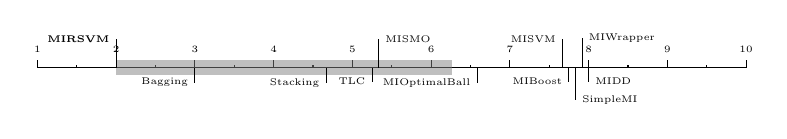
\begin{tikzpicture}
\draw (1,0) -- (10,0);
\foreach \x in {1,2,3,4,5,6,7,8,9,10} {
\draw (\x, 0) -- ++(0,.1) node [above,scale=0.7] {\tiny \x};
\ifthenelse{\x < 10}{\draw (\x+.5, 0) -- ++(0,.03);}{}
}

\coordinate (c0) at (2,0);
\coordinate (c1) at (7.75,0);
\coordinate (c2) at (6.5833,0);
\coordinate (c3) at (8,0);
\coordinate (c4) at (7.9167,0);
\coordinate (c5) at (5.3333,0);
\coordinate (c6) at (7.6667,0);
\coordinate (c7) at (7.8333,0);
\coordinate (c8) at (5.25,0);
\coordinate (c9) at (3,0);
\coordinate (c10) at (4.6667,0);

\node (l0) at (c0) [above left=.23cm and 0cm, align=right,scale=0.7] {\tiny \textbf{MIRSVM}};
\node (l1) at (c1) [below left=.05cm and 0cm, align=right,scale=0.7] {\tiny MIBoost};
\node (l2) at (c2) [below left=.05cm and 0cm, align=right,scale=0.7] {\tiny MIOptimalBall};
\node (l3) at (c3) [below right=.05cm and 0cm, align=right,scale=0.7] {\tiny MIDD};
\node (l4) at (c4) [above right=.23cm and 0cm, align=right,scale=0.7] {\tiny MIWrapper};
\node (l5) at (c5) [above right=.23cm and 0cm, align=right,scale=0.7] {\tiny MISMO};
\node (l6) at (c6) [above left=.23cm and 0cm, align=right,scale=0.7] {\tiny MISVM};
\node (l7) at (c7) [below right=.27cm and 0cm, align=right,scale=0.7] {\tiny SimpleMI};
\node (l8) at (c8) [below left=.05cm and 0cm, align=right,scale=0.7] {\tiny TLC};
\node (l9) at (c9) [below left=.05cm and 0cm, align=right,scale=0.7] {\tiny Bagging};
\node (l10) at (c10) [below left=.05cm and 0cm, align=right,scale=0.7] {\tiny Stacking};

\fill[fill=gray,fill opacity=0.5] (2,-0.1) rectangle (6.26,0.1);

\foreach \x in {0,1,2,3,4,5,6,7,8,9,10} {
\draw (l\x) -| (c\x);
};
\end{tikzpicture}}
\captionof{figure}{Bonferroni-Dunn test for overall ranks comparison}\label{fig:BonfDunnpmeta}
\end{table}

\subsection{Overall Comparison}
Table~\ref{tab:time} shows the run time results, in seconds, for each algorithm. MIRSVM has the fastest run time and is ranked second. MIRSVM shows very good scalability considering the number of features, such as in the webmining dataset which comprises of $5863$ attributes. Additionally, taking into account the number of instances as seen in the two largest datasets, component and function, MIRSVM displays superior scalability. It is important to note that quadratic programming solvers are not the most efficient tools for solving optimization problems in terms of run time, and yet MIRSVM still is shown to perform competitively against the current state-of-the-art algorithms. 

SimpleMI achieves the highest rank and competitive run times because, rather than use the instances in each bag to train a model, it takes the mean value of the instances in a bag and uses that for training. Even though SimpleMI has fast run-times, its performance over the previous metrics has been shown to be random and not as efficient as the bag-level methods.

Table~\ref{tab:metarank} shows the ranks achieved by each of the metrics along with the average and meta-ranks. MIRSVM has the best meta-rank (rank of the ranks) and the Bagging ensemble method has the next best. The meta-ranks also highlight the better performance of bag-level methods over instance-level and wrapper methods, emphasizing the importance of training at the bag-level. Not only does MIRSVM use bag-level information during classification, but it also optimizes over the instances within the bag, which helps determine which instances contribute the most information about the bags label. SimpleMI, MIWrapper, MIBoost, MISVM, MIOptimalBall, and MDD have the worst performance compared to MIRSVM and Bagging. Although these algorithms are popular in literature, the experimental study clearly shows that recent bag-level and ensemble methods easily overcome traditional multi-instance learning algorithms. 

In summary, MIRSVM offers improvement in terms of both accuracy and run-time when compared to referenced methods, especially those utilizing SVM-based algorithms.

\section{Conclusion}\label{sec:conclusion}
This paper proposed a novel formulation and algorithm for the multiple-instance support vector machine problem, which optimizes bags classification via bag-representative selection. First, the primal formulation was posed and its dual was then derived and computed using a quadratic programming solver. This formulation was designed to utilize bag-level information and find an optimal separating hyperplane between bags, rather than individual instances, using the standard multi-instance assumption. The SMI assumption states that a bag is labeled positive if and only if at least one instance within a bag is positive, and is negative otherwise. The key features of the proposed algorithm MIRSVM are its ability to identify instances within positive and negative bags, i.e. the support vectors or representatives, that highly impact the decision boundaries as well as avoiding uncertainties and issues caused by techniques that flatten, subset, or under-represent positive instances within positively labeled bags. Additionally, it exhibits desirable scalability, making it suitable for large-scale learning tasks.

The experimental study showed the better performance of MIRSVM compared with multi-instance support vector machines, traditional multi-instance learners, as well as with ensemble methods. The results, according to a variety of performance metrics, were compared and further validated using statistical analysis with non-parametric tests which highlight the advantages of using bag-level based and ensemble learners such as Bagging and Stacking, while showing the instance-level based learners performed poorly in comparison or were deemed as strongly biased and unstable classifiers. On the contrary, our proposal MIRSVM performs statistically better, neither compromising accuracy nor run-time while displaying a robust performance across all of the evaluated datasets.

\begin{acknowledgements}
This research was supported by the Spanish Ministry of Economy and Competitiveness, project TIN2014-55252-P, and by FEDER funds.
\end{acknowledgements}

% BibTeX users please use one of
\bibliographystyle{natbib}
\bibliography{references}   

\end{document}


